\documentclass[11pt,english,french]{scrreprt}
\usepackage{lmodern}
\usepackage{babel}
\renewcommand{\familydefault}{\rmdefault}
\usepackage[T1]{fontenc}
\usepackage{ucs}
\usepackage[utf8x]{inputenc}
\usepackage[a4paper]{geometry}
\geometry{verbose,tmargin=3cm,bmargin=3cm,lmargin=2cm,rmargin=2cm,headheight=2cm,footskip=2cm}
\setlength{\parskip}{\smallskipamount}
\setlength{\parindent}{0pt}

\usepackage[titles]{tocloft}
\usepackage{abstract}
\usepackage{amsthm}
\usepackage{booktabs}
\usepackage{amsmath}
\usepackage{amssymb}
\usepackage[unicode=true, pdfusetitle,
 bookmarks=true,bookmarksnumbered=false,bookmarksopen=false,
 breaklinks=false,pdfborder={0 0 1},backref=false,colorlinks=false]
 {hyperref}

\makeatletter
\usepackage{colortbl}
\usepackage{color}
\usepackage[dvipsnames]{xcolor}
\usepackage{listings}
\usepackage[calcwidth]{titlesec}
\usepackage{fix-cm}
\usepackage{multicol}
\usepackage{wrapfig}
\usepackage{graphicx}
\usepackage{tabularx}
\graphicspath{{images/}}
\usepackage{algorithm,algorithmic}
\usepackage{nicefrac}
\usepackage{verbatim}
\usepackage{moreverb}
\usepackage{subfig}
\usepackage[strict]{changepage}

\theoremstyle{remark}
  \newtheorem*{rem*}{Remarque}
  \newtheorem*{ex*}{Exemple}
\theoremstyle{definition}
  \newtheorem*{def*}{Définition}
  \newtheorem*{obj*}{Objectif}
  \newtheorem*{idee*}{Idée}

\definecolor{MyDarkBlue}{rgb}{0,0.08,0.45}

\lstset{language=C,
	 	basicstyle=\small\ttfamily,
		keywordstyle=\ttfamily\textcolor{RubineRed},
		identifierstyle=,
		commentstyle=\textcolor{OliveGreen},
		columns=fullflexible,
		stringstyle=\sffamily,
		showstringspaces=false,numberstyle=\tiny, breaklines=true}

\titleformat{\section}[hang]{\sffamily\bfseries}
 {\Large\thesection}{12pt}{\Large}[{\titlerule[0.5pt]}]

\titleformat{\subsection}[hang]{\sffamily\bfseries}
 {\large\thesubsection}{12pt}{\large}

\def\thickhrulefill{\leavevmode \leaders \hrule height 1pt\hfill \kern \z@}

\makeatletter
\def\maketitle{%
  \null
  \thispagestyle{empty}%
  \vfill
  \begin{center}\leavevmode
    \normalfont
    {\huge \sffamily \bfseries\color{orange}\raggedright \@title\par}%
    \thickhrulefill\par
    {\large\sffamily\color{MyDarkBlue}\raggedleft \@author\par}%
    \vskip 1cm
    {\Large \sffamily \@date\par}%
	{\Large \sffamily \@blurb\par}%
  \end{center}%
  \vfill
  \null
  \cleardoublepage
  }

\def\blurb#1{\def\@blurb{#1}}

\AtBeginDocument{
  \def\labelitemi{\normalfont\bfseries{--}}
}
\renewcommand{\abstractname}{Introduction}
\renewcommand{\abstractnamefont}{\Large\sffamily\bfseries}
\renewcommand{\absnamepos}{flushleft}

\setlength{\cftbeforesecskip}{0.5ex}
\setlength{\cftbeforepartskip}{2ex}
\setlength{\cftsecindent}{1cm}
\renewcommand{\cftsecfont}{\mediumsize \sffamily \bfseries}
\renewcommand{\cftsecdotsep}{\cftdotsep}


\setcounter{tocdepth}{1}

\usepackage{remreset}
\makeatletter 
\@addtoreset{section}{part}
\@addtoreset{section}{chapter} 
\makeatother

\def\@part[#1]#2{%
      \ifnum \c@secnumdepth >\m@ne
        \refstepcounter{part}%
        \addcontentsline{toc}{part}{\thepart\hspace{1em}#1}%
      \else
        \addcontentsline{toc}{part}{#1}%
      \fi
      {\parindent \z@ \raggedright
       \interlinepenalty \@M
       \normalfont
       \ifnum \c@secnumdepth >\m@ne
         \Large \sffamily \bfseries \partname~\thepart
         \par\nobreak
       \fi
       \huge \sffamily \bfseries #2%
       \markboth{}{}\par}%
      \nobreak
      \vskip 5ex
      \@afterheading}
  \def\@spart#1{%
      {\parindent \z@ \raggedright
       \interlinepenalty \@M
       \normalfont
       \huge \sffamily \bfseries #1\par}%
       \nobreak
       \vskip 3ex
       \@afterheading}

\makeatother

\makeatletter
\def\@makechapterhead#1{%
  \vspace*{10\p@}%
  {\parindent \z@ \raggedright
    \normalfont
    \ifnum \c@secnumdepth >\m@ne
      \if@mainmatter
        %\huge\bfseries 
        \scshape
        \@chapapp\space \thechapter
        \par\nobreak
%        \vskip 20\p@
      \fi
    \fi
    \interlinepenalty\@M
    \Huge \bfseries \sffamily #1\par\nobreak
    \vskip 40\p@
  }}
\def\@schapter#1{\if@twocolumn
                   \@topnewpage[\@makeschapterhead{#1}]%
                 \else
                   \@makeschapterhead{#1}%
                   \@afterheading
                 \fi}
\def\@makeschapterhead#1{%
  \vspace*{10\p@}%
  {\parindent \z@ \raggedright
    \normalfont
    \scshape
    \interlinepenalty\@M
    \Huge \bfseries \sffamily #1\par\nobreak
    \vskip 40\p@
  }}

\makeatother

%%% francisation des algorithmes
\renewcommand{\algorithmicrequire} {\textbf{\textsc{Entrées :}}}
\renewcommand{\algorithmicensure}  {\textbf{\textsc{Sorties :}}}
\renewcommand{\algorithmicwhile}   {\textbf{tant que}}
\renewcommand{\algorithmicdo}      {\textbf{faire}}
\renewcommand{\algorithmicendwhile}{\textbf{fin tant que}}
\renewcommand{\algorithmicend}     {\textbf{fin}}
\renewcommand{\algorithmicif}      {\textbf{si}}
\renewcommand{\algorithmicendif}   {\textbf{fin si}}
\renewcommand{\algorithmicelse}    {\textbf{sinon}}
\renewcommand{\algorithmicthen}    {\textbf{alors}}
\renewcommand{\algorithmicfor}     {\textbf{pour}}
\renewcommand{\algorithmicforall}  {\textbf{pour tout}}
\renewcommand{\algorithmicdo}      {\textbf{faire}}
\renewcommand{\algorithmicendfor}  {\textbf{fin pour}}
\renewcommand{\algorithmicloop}    {\textbf{boucler}}
\renewcommand{\algorithmicendloop} {\textbf{fin boucle}}
\renewcommand{\algorithmicrepeat}  {\textbf{répéter}}
\renewcommand{\algorithmicuntil}   {\textbf{jusqu'à}}
\renewcommand{\algorithmicreturn}   {\textbf{retourner}}

\floatname{algorithm}{Algorithme}

\let\mylistof\listof
\renewcommand\listof[2]{\mylistof{algorithm}{Liste des algorithmes}}

% pour palier au problème de niveau des algos
\makeatletter
\providecommand*{\toclevel@algorithm}{0}
\makeatother

%\listofalgorithms % pour lister les algos (après la toc)



\begin{document}
\author{BARON Benjamin }
\date{Le \today}
\blurb{D'après le cours de \href{http://www-asim.lip6.fr/~alain/}{Alain Greiner}}

\title{LI312 - Cours\\
Architecture logicielle et matérielle des ordinateurs}

\maketitle
\renewcommand\contentsname{} 
\tableofcontents

\chapter{Architecture externe du processeur MIPS32} % (fold)

\section{Introduction} % (fold)

Le processeur lit (fetch) le code d'instruction qu'il doit exécuter.\\
Il est alors capable de lire une instruction par cycle.

La valeur 32 bits fait référence à :\begin{itemize}
	\item La taille de l'adresse (adresse codée sur 32 bits) ;
	\item La capacité de stockage interne du processeur (ie. La capacité des registres).
\end{itemize}

\begin{figure}[!h]
	\center
	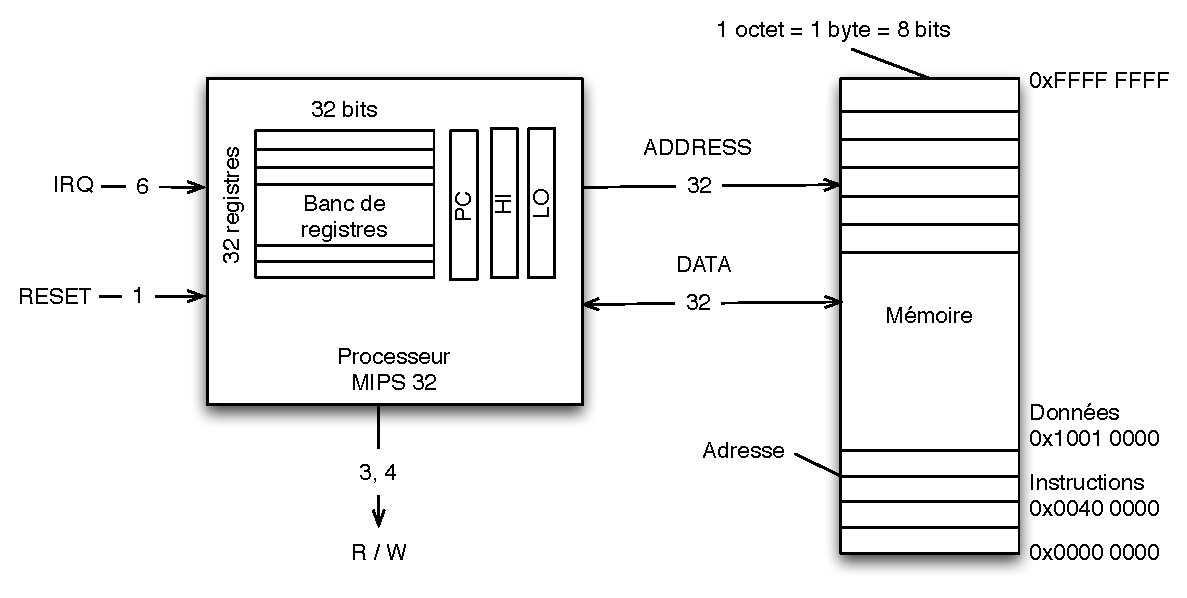
\includegraphics[scale=.5]{diagrammes/MIPS32}
	\caption{Schéma du processeur MIPS 32}
\end{figure}

\begin{rem*}
	Le MIPS est un processeur RISC (\emph{Reduced Instruction Set Computer}) $\neq$ CISC (\emph{Complex Instruction Set Computer}). Les instructions que le processeur manipule comportent 3 registres : 2 registres sources et un registre destination. De ce fait, il faut un même nombre de cycles pour exécuter chaque instruction du jeu d'instruction. Il est donc possible de débuter une instruction à chaque cycle d'horloge (\emph{pipeline}).
\end{rem*}

Entrées / sorties du processeur :\begin{itemize}
	\item ADDRESS sur 32 bits en sortie ;
	\item DATA sur 32 bits en entrée / sortie ;
	\item Read / Write généralement sur 3 ou 4 bits, en sortie ;
	\item IRQ sur 6 bits en entrée -- permet à un périphérique de déclencher une interruption ;
	\item RESET sur 1 bit en entrée -- permet initialisation (ie. Mettre la machine dans un état connu).
\end{itemize}

\vspace{10pt}

Il existe différents types de registres.

Registres internes visibles du logiciel :\begin{itemize}
	\item 32 registres généraux sur 32 bits (notés $R(i)$ pour $i\in[0,\,31]$) ;
	\item PC : Program Counter -- sauvegarde la position de la dernière instruction exécutée ;
	\item HI et LO -- utilisés pour les opérations arithmétiques $+$ et $/$. 
\end{itemize}

\vspace{10pt}

Registres protégés -- non accessibles en mode utilisateur, seulement en mode superviseur:\begin{itemize}
	\item SR : Status Register sur 2 bits :\begin{itemize}
		\item Processeur en mode user / root ;
		\item Interruptions masquées ou non.
	\end{itemize}
	\item CR : Cause Register :\begin{itemize}
		\item Interruption matérielle = message d'un périphérique à un logiciel ;
		\item Exception : programme utilisateur fait quelque chose d'interdit $\Rightarrow$ programme tué, dénonciation de la cause de l'erreur ;
		\item Appel système : appel à l'OS (eg. Ecriture disque).
	\end{itemize}
	\item EPC : Exception Program Counter -- pour les interruptions matérielles et les exceptions ;
	\item BAR : Bad Address Register -- Erreur d'adressage (eg. segmentation fault) ;
	\item PROCID : Numéro de processeur : identifiant du processeur (utile pour les processeurs multi-core) ;
	\item CYCLECOUNT : compteur de cycles.
\end{itemize}

\vspace{10pt}

Il y a deux modes de fonctionnement du processeur : \begin{itemize}
	\item mode utilisateur ;
	\item mode superviseur (mode \emph{kernel}).
\end{itemize}

\begin{rem*}
	Le matériel surveille en permanence le logiciel en train de s'exécuter. S'il tente d'accéder à une zone protégée, le matériel va lever une exception. 
\end{rem*}

\section{Communication avec la mémoire} % (fold)
La mémoire est un tableau d'octets (à l'image d'une commode et de ses tiroirs). 

\begin{figure}[!h]
	\center
	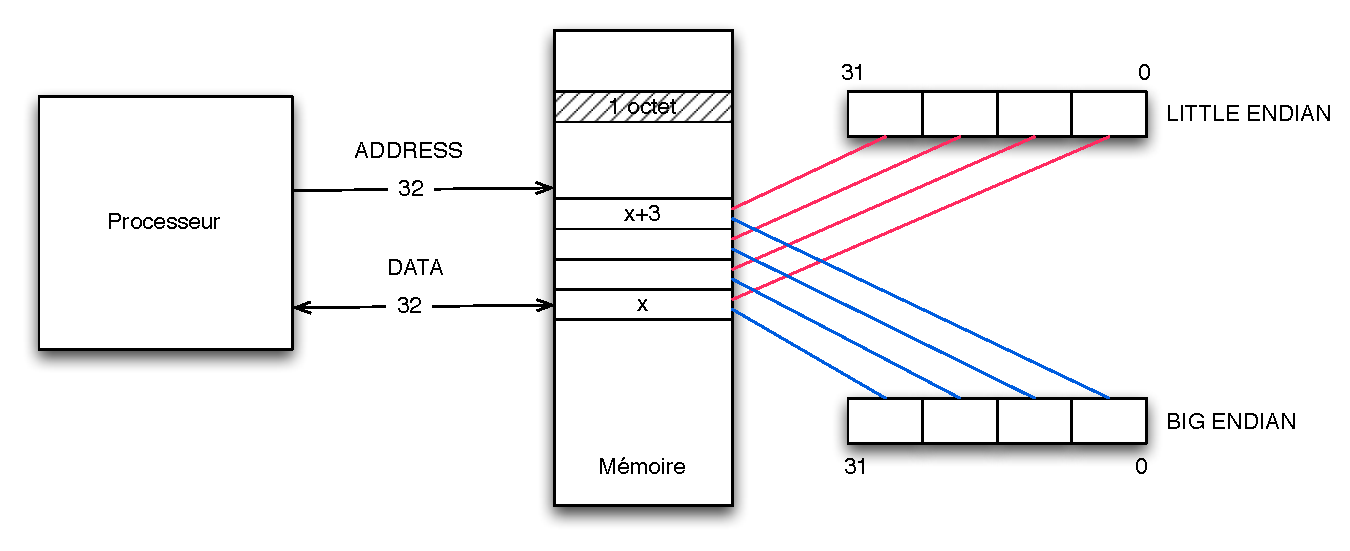
\includegraphics[scale=.5]{diagrammes/Memoire1}
	\caption{Communication avec la mémoire}
\end{figure}

\begin{rem*}
	Lorsque l'instruction exécutée par le processeur cherche à lire un mot (ie. un ensemble de 32 bits alignés), l'adresse \textbf{doit} être un multiple de 4 (ie. de la forme 0x------00).
	
	Dans le cours nous utiliserons la disposition \emph{little endian} : l'adresse la plus petite correspond à l'octet le plus petit (de poids faible).
\end{rem*}

L'adressage est divisé en deux zones :\begin{itemize}
	\item La zone utilisateur (\emph{user});
	\item La zone superviseur (\emph{kernel}).
\end{itemize}

\begin{rem*}
	Chaque fois que le logiciel demande au processseur d'exécuter une instruction qui accède au segment superviseur, le matériel vérifie que le bit de mode du registre STATUS REGISTER (SR) à la valeur \emph{superviseur}.
\end{rem*}

\vspace{20pt}

\begin{figure}[h!]
	\center
	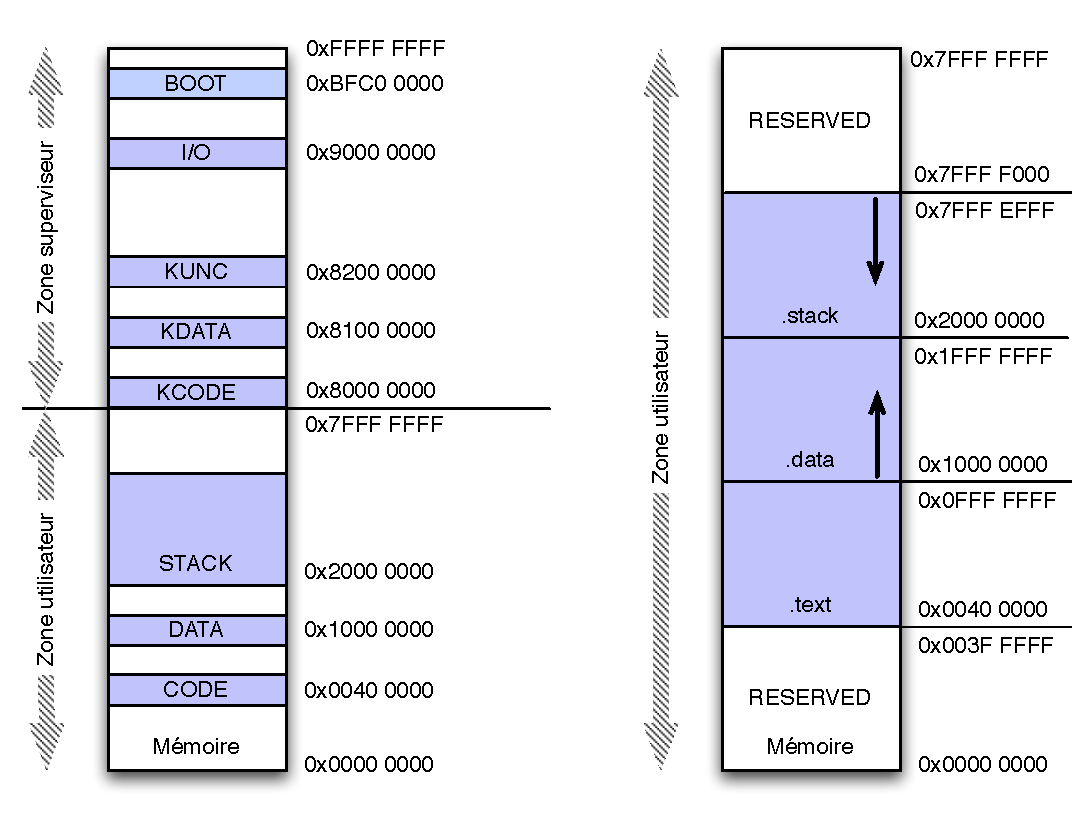
\includegraphics[scale=.5]{diagrammes/Memoire2}
	\caption{Segmentation de la mémoire}
\end{figure}

Segments réservés de la partie superviseur : \begin{itemize}
	\item \textbf{Code de BOOT} : code qu'exécute la machine lors du démarrage / reset de la machine. Ce code est situé dans la mémoire ROM (ie. mémoire morte) et constitue le BIOS ;
	\item \textbf{KCODE} : code protégé du système d'exploitation. Le BIOS lit sur le disque le code du système d'exploitation et le range dans cet espace mémoire (lors du boot de la machine) ;
	\item \textbf{KDATA} : données globales privées de l'OS -- tables contenant les contextes d'exécution des tâches en mode multiprocesseur notamment ;
	\item \textbf{UNC} : données non cachables (ie. les valeurs ne sont pas recopiées dans le cache). Ce sont des tampons de communication entre le processeur et les périphériques ;
	\item \textbf{I/O} : contrôleur des périphériques. Un périphérique peut être partagé par plusieurs utilisateurs différents. I/O est alors dans la partie superviseur de l'espace adressable.
\end{itemize}

\vspace{10pt}

Segments réservés de la partie utilisateur :\begin{itemize}
	\item \textbf{CODE} : code du programme utilisateur, ainsi que le code des fonctions permettant à un programme utilisateur d'accéder aux périphériques grâce aux appels systèmes ;
	\item \textbf{DATA} : données globales du programme utilisateur ;
	\item \textbf{STACK} : pile d'exécution du programme.
\end{itemize}


\begin{rem*}
	Des espaces adressables sont câblés en dur dans le matériel :\begin{itemize}
		\item Le segment BOOT (0xBFC0 0000). Cette adresse câblée est commune à tous les processeurs ;
		\item La séparation mode superviseur (2 Go) / mode utilisateur (2 Go) pour un processeur sans mémoire virtuelle.
	\end{itemize}
\end{rem*}

\section{Format des instructions} % (fold)

Toutes les instructions (jeux d'instructions) sont codées sur 32 bits (alignés en mémoire).

\begin{rem*}
	Vrai pour le MIPS R3000, mais par exemple pour les processeur x86 d'Intel, il y a la possibilité d'avoir des instructions codées sur 1, 2, 4, 6, 8 octets.
\end{rem*}

Il y a 3 sous-formats :\begin{itemize}
	\item Le \textbf{format R} est utilisé par les instructions nécessitant 2 registres sources (désignés par RS et RT) et un registre résultat désigné par RD (\lstinline!add!, \lstinline!or!\dots) ;
	\item Le \textbf{format I} est utilisé par les instructions de lecture/écriture mémoire (\lstinline!lw! et \lstinline!sw!), par les instructions utilisant un opérande immédiat (\lstinline!addi!, \lstinline!andi!\dots), ainsi que par les branchements courte distance (conditionnels) (\lstinline!bne!, \lstinline!beq!\dots) ;
	\item Le \textbf{format J} n’est utilisé que pour les branchements à longue distance (inconditionnels) (\lstinline!jal!, \lstinline!j!\dots).
\end{itemize}
\begin{figure}[!h]
	\center
	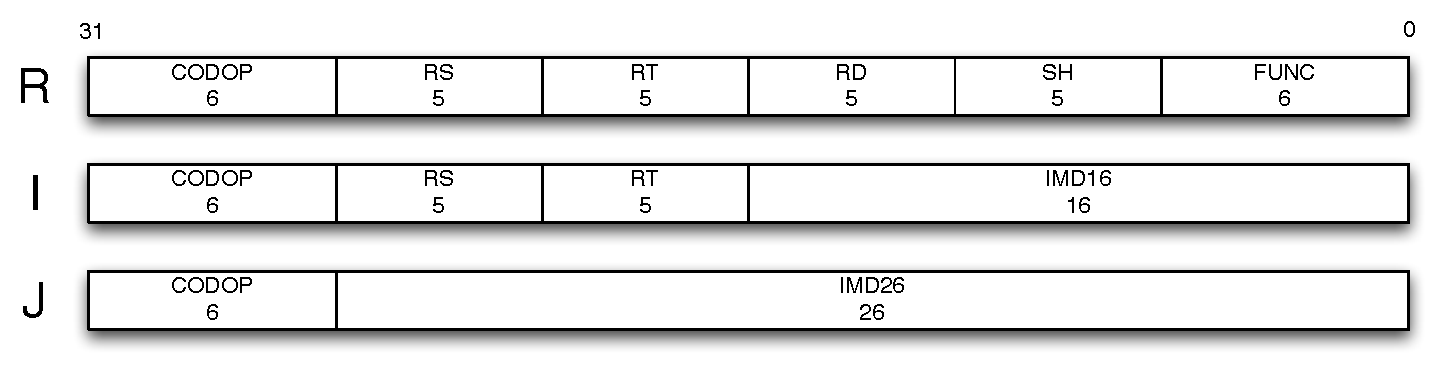
\includegraphics[scale=.5]{diagrammes/Format}
	\caption{Formats d'instructions du MIPS 32}
\end{figure}

\begin{def*}[Valeur immédiate]
	Valeur que l'instruction va utiliser comme opérande sans avoir à la lire dans un registre ou en mémoire.
\end{def*}


\section{Conventions d'utilisation de la pile d'exécution} % (fold)

On souhaite utiliser les conventions utilisées par GCC.

Les 3 fonctions de la pile :\begin{enumerate}
	\item Transmission des arguments de la fonction appelante vers la fonction appelée ;
	\item Sauvegarde de la valeur des « registres persistants » ;
	\item Zone de travail : variables locales.
\end{enumerate}

\begin{rem*}
	Les deux instructions permettant d'appeler une fonction :\begin{itemize}
		\item jal PC $\leftarrow$ IMD26\\
		R(31) $\leftarrow$ PC + 4
		\item bgezal PC $\leftarrow$ IMD26\\
		R(31) $\leftarrow$ PC + 4
	\end{itemize}
\end{rem*}

Par convention, on utilise le registre R(29) comme pointeur de pile (\emph{Stack Pointer}). Le pointeur de pile pointe sur les dernières case occupées dans la pile.\\
La pile est remplie à partir de l'adresse 0x7FFF EFFF et utilise un système d'adressage \emph{décroissant}.

\begin{figure}[!h]
	\vspace{-10pt}
	\center
	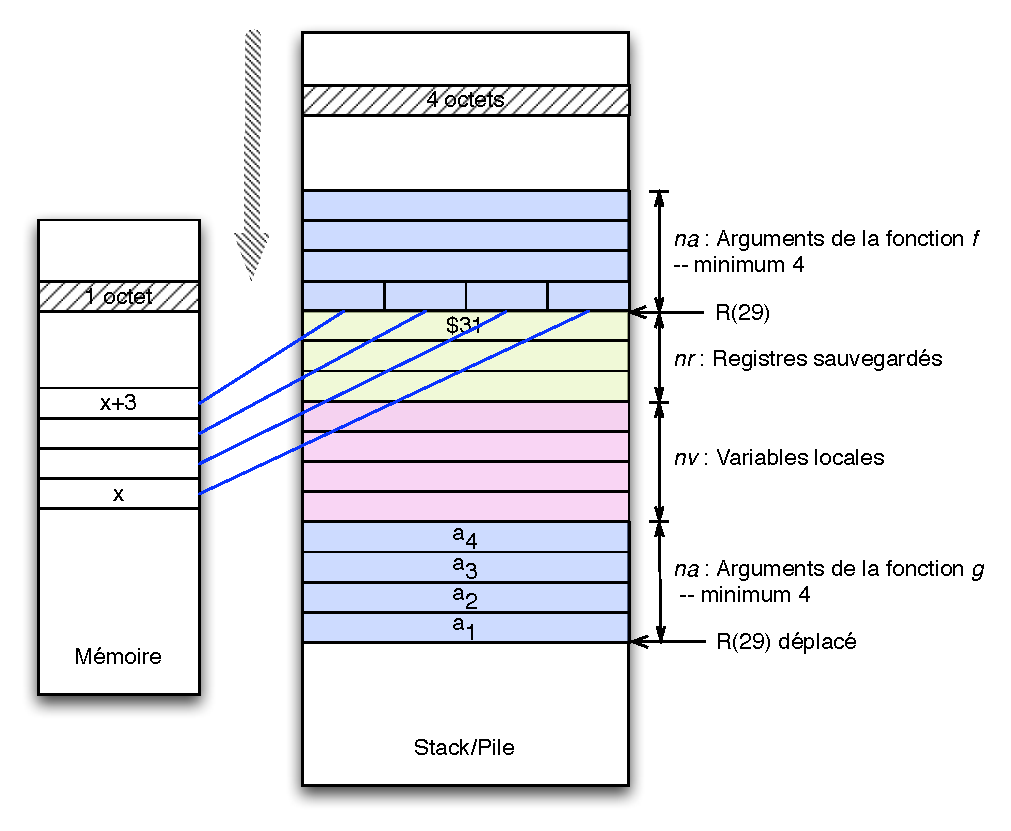
\includegraphics[scale=.48]{diagrammes/Stack}
	\vspace{-10pt}
	\caption{Schéma de la pile d'exécution}
	\vspace{-20pt}
\end{figure}

\vspace{20pt}

On a alors :\begin{itemize}
	\item $na=\max(na_i,\,4)$ où $na_i$ représente ne nombre d'arguments des fonctions $g_i$ appelées par $f$ ;
	\item $nv$ est le nombre de variables locales utilisées en C ;
	\item $nr$ est le nombre de registres persistants utilisés $+$ \$31.
\end{itemize}

\begin{def*}[Registres persistants et registres temporaires]
	On distingue deux catégories de registres :\begin{itemize}
		\item Les registres \textbf{persistants} : sauvegarder leur état initial dans la pile avant l'exécution d'une fonction, puis restaurer l'état initial de ces registres à la fin de l'exécution de la fonction.\\
		$\Rightarrow$ Registres \$16 à \$23 et \$28 à \$31 ;
		\item Les registres \textbf{temporaires} : à ne pas sauvegarder dans la pile. Une fonction peut les modifier sans en restaurer la valeur initiale.\\
		$\Rightarrow$ Registres \$1 à \$15 et \$24, \$25 ;
		\item Les registres \textbf{réservés} au système d'exploitation : non utilisables par les applications utilisateur.\\
		$\Rightarrow$ Registres \$0, \$26 et \$27.
	\end{itemize}
	\begin{figure}[!h]
		\vspace{-10pt}
		\center
		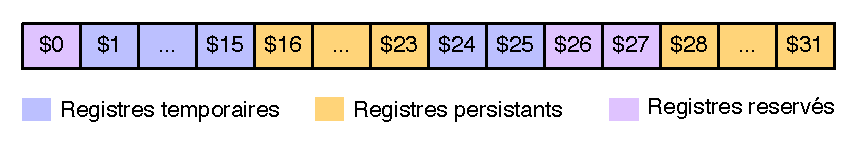
\includegraphics[scale=.5]{diagrammes/registres}
		\vspace{-15pt}
	\end{figure}
\end{def*}

\begin{rem*}
	Utilité de réserver des places dans la pile pour les variables locales $(nv)$ :\begin{itemize}
		\item Ca ne coûte pas cher en mémoire : on re-libère la mémoire à la fin de l'exécution de la fonction ;
		\item Si il y a des variables locales de tailles importantes (eg. des tableaux), on utilise la mémoire réservée dans la pile pour les stocker temporairement.
	\end{itemize}
\end{rem*}

\section{Optimisations de GCC} % (fold)
Le compilateur GCC opère au minimum deux optimisations.

\textbf{La première.} Distinguer les registres persistants (\$16 à \$23) des registres à vie courte. De ce fait, on va sauvegarder leur valeur dans la pile.

\textbf{La seconde.} Passage des arguments par registres. En effet, la transmission des arguments par la pile (mémoire) coûte cher en utilisation du processeur : \begin{itemize}
	\item Si les valeurs cherchées se trouvent dans le cache, c'est OK (environ 1 cycle) ;
	\item Si les valeur cherchées ne se trouvent pas dans le cache, il va falloir aller les chercher en mémoire (environ 400 cycles).
\end{itemize}
\textbf{Objectif.} Amélioration des performances.

Quand il y a moins de 5 arguments (de 1 à 4), GCC écrit la valeur des arguments dans les registres \$4, \$5, \$6 et \$7.

Il n'écrit pas les valeurs de ces 4 premiers arguments, mais réserve leur place dans la pile quand même, en plus de réserver une place dans la pile pour les autres arguments.
\[
	f(\underbrace{a_{1},\, a_{2},\, a_{3},\, a_{4}}_{\$4,\;\$5,\;\$6,\;\$7},\,\underbrace{a_{5},\,\dots,\, a_{n}}_{\textrm{pile}})
\]

\begin{rem*}
	Si une fonction $f$ a au moins 4 arguments, elle en transmet 4 par registre et réserve leur place dans la pile. Si cette fonction appelle une autre fonction $g$. De ce fait, $f$ va sauvegarder la valeur des registres \$4 à \$7 à leur place appropriée dans la pile pour continuer à utiliser les valeurs des arguments.
\end{rem*}

\vfill

\section{Organisation générale d'une chaîne de compilation -- GCC} % (fold)

On utilise 4 outils :\begin{itemize}
	\item assembleur \emph{as} : \lstinline!mipsel-li321-elf-as! ;
	\item compilateur \emph{gcc} : \lstinline!mipsel-li321-elf-gcc! ;
	\item linker \emph{ld} : \lstinline!mipsel-li321-elf-ld! ;
	\item désassembleur \emph{objdump} : \lstinline!mipsel-li321-elf-objdump!.
\end{itemize}

\begin{rem*}
	Le nom \lstinline!mipsel-li321-elf-XX! correspond à :\begin{itemize}
		\item \lstinline!mpisel! : processeur MIPS, Little Endian ;
		\item \lstinline!li321! : nom du système qui s'exécute ;
		\item \lstinline!elf! : le code binaire généré respecte le format elf ;
		\item \lstinline!XX! : outil utilisé.
	\end{itemize}
\end{rem*}

\begin{figure}[h!]
  \centering
  \subfloat[Chaîne de compilation]{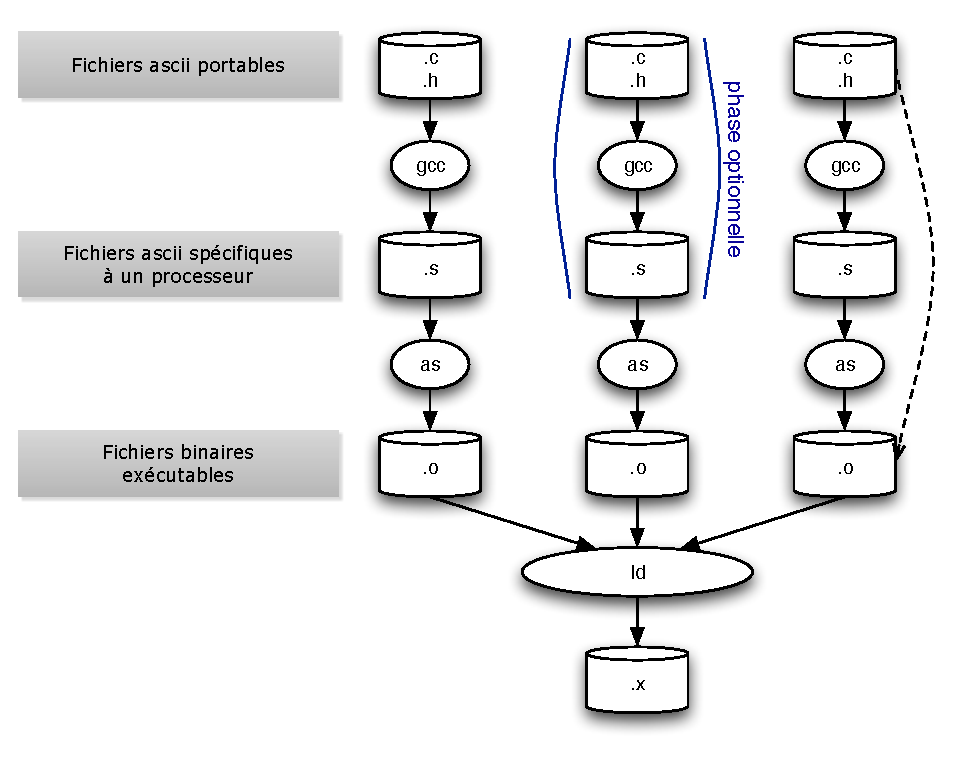
\includegraphics[width=0.5\textwidth]{diagrammes/Compilation}}\qquad            
  \subfloat[Phase de décompilation --- débogage]{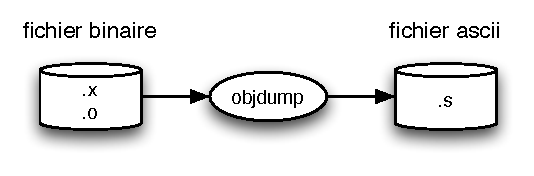
\includegraphics[width=0.35\textwidth]{diagrammes/compilation2}}
\end{figure}

La compilation séparée est possible. Les fonctions d'un fichier peuvent faire référence (via des adresses mémoires) à des fonctions issues d'autres fichiers.

L'édition de liens (ld) résout les adresses : assigner des valeurs binaires aux valeurs symboliques des adresses (labels).\\
Les valeurs non résolues dans les fichiers binaires sont stockées dans des tables de symboles. On remplace alors les adresses non résolues à la fin de la chaine de compilation.

Les différents modules logiciels qui vont être exécutés n'entrent pas forcément dans la chaîne de compilation au niveau du fichier \lstinline!*.c!. On a la possibilité de compiler à la fois des fichiers \lstinline!*.h!/\lstinline!*.c! et \lstinline!*.s!.


Comment contrôler cette chaîne de compilation ?

Via l'édition de liens principalement : donner au programme d'éditeur de liens des consignes d'exécution :\begin{itemize}
	\item Chaque fichier objet (\lstinline!*.o!) contient une ou plusieurs section (eg. section \lstinline!.data!, \lstinline!.text! dans un fichier assembleur).
	
	On peut guider le linker pour qu'il regroupe une ou plusieurs \emph{section} dans un \emph{segment} (KCODE, KDATA, DATA, CODE\dots) de l'espace adressable.
	
	\begin{ex*}
		Regrouper le contenu de la section \lstinline!.text! des différents fichiers objets (\lstinline!*.o!) dans le segment CODE de l'espace adressable.
	\end{ex*}
	\item On peut définir les adresses de base des différents segments cibles.
\end{itemize} 

\chapter{Bus système} % (fold)

\section{Introduction} % (fold)

Le programme s'exécutant sur le processeur peut accéder à différents services via le bus système. Ce dernier permet la communication du processeur avec le monde extérieur.

\begin{figure}[!h]
	\center
	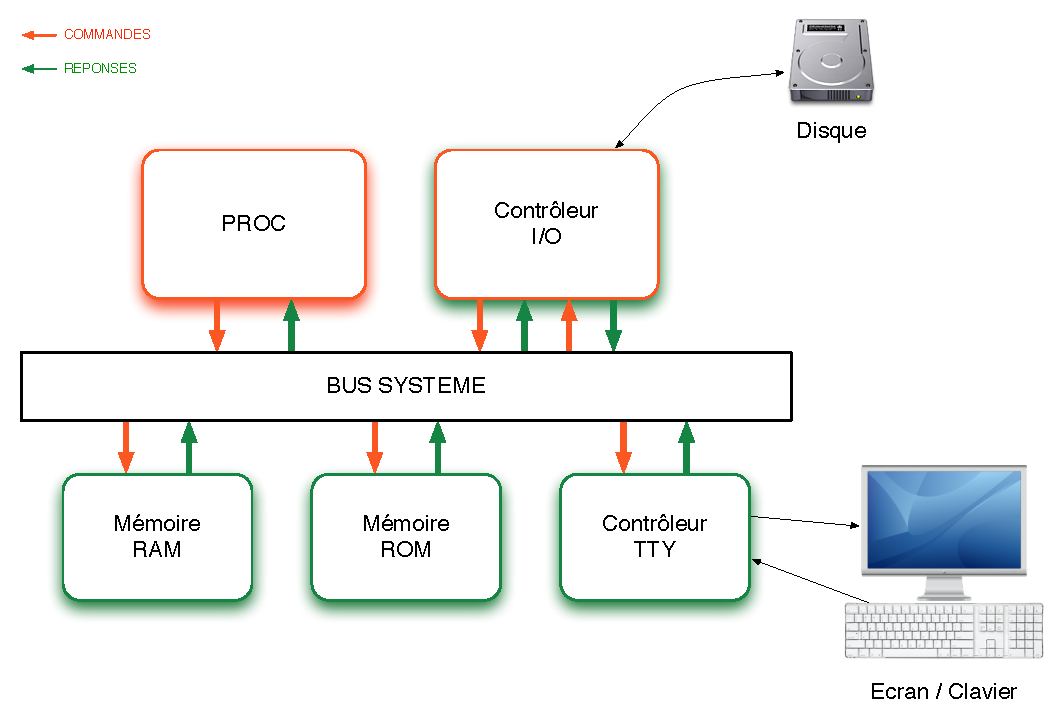
\includegraphics[scale=.75]{diagrammes/Bus1}
	\caption{Représentation de la machine dans son ensemble}
\end{figure}

\begin{def*}[Transaction]
	Echange d'informations en utilisant le bus système. Il s'agit d'une écriture (\lstinline!sw!), ou d'une lecture (\lstinline!lw!) à une certaine adresse.
	
	Toujours une paire :\begin{itemize}
		\item Une commande ;
		\item Une réponse.
	\end{itemize}
\end{def*}

\begin{rem*}
	Il existe une réponse même dans le cas d'une commande écriture.
	
	Le processeur peut commander une écriture vers autre chose qu'une mémoire. Il peut exécuter cet ordre sur un périphérique.
\end{rem*}

\begin{def*}[Maître / Initiateur]	
	Composant matériel capable de démarrer une transaction (ie. envoyer une commande).
\end{def*}

\begin{def*}[Esclave / Cible]
	Composant matériel capable de recevoir une commande et d'y répondre.
\end{def*}

\begin{rem*}
	Attention : un même composant matériel peut être à la fois maître et esclave.
	
	Par exemple : le contrôleur de disque : Disque $\longleftrightarrow$ Mémoire RAM.\\
	Il a besoin d'adresser la mémoire pour lire / écrire dans celle-ci.
\end{rem*}


\section{Services offerts par le bus système} % (fold)

Hypothèse. Le bus système n'exécute qu'une seule transaction à la fois.

\begin{figure}[!h]
	\center
	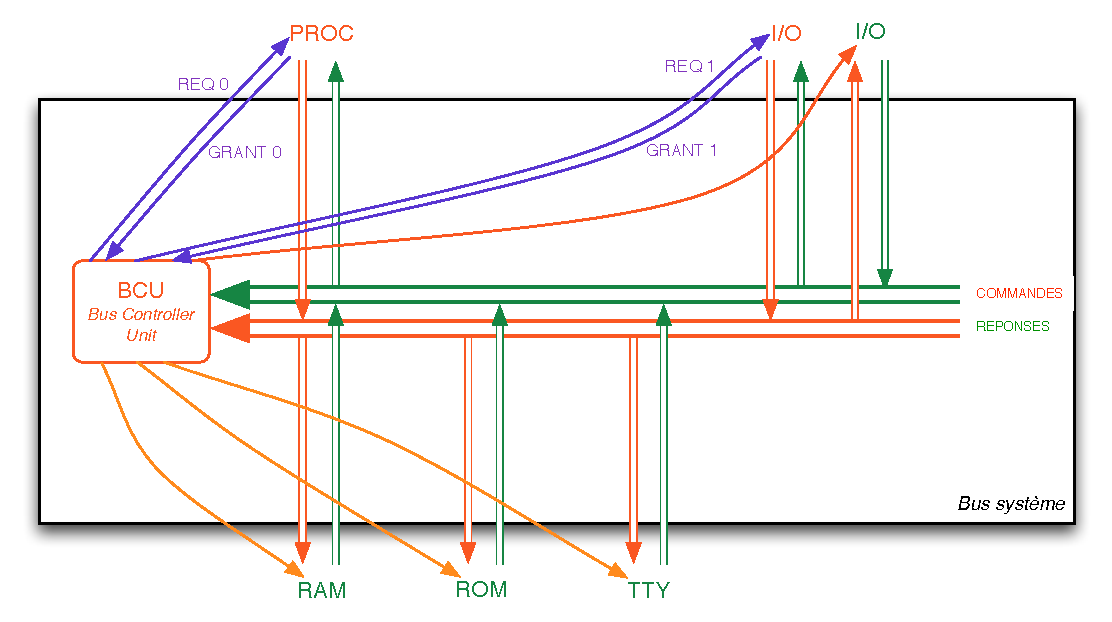
\includegraphics[scale=.75]{diagrammes/Bus2}
	\caption{Le bus système}
\end{figure}

\subsection*{Arbitrage entre les différents maîtres} % (fold)
Le bus système est une ressource partagée entre au moins deux maîtres.

Du fait du parallélisme et des requêtes asynchrones provenant de différents entités, des collisions apparaissent. Un arbitrage est nécessaire.

Deux maîtres veulent utiliser en même temps le bus système. Il faut donc assurer un mécanisme d'arbitrage pour accéder à la ressource partagée (ici : le bus d'adresse).

Déroulement d'une transaction :\begin{itemize}
	\item Request : avant d'émettre une transaction, l'initiateur demande l'autorisation d'émettre au BCU (\emph{Bus Controller Unit});
	\item Grant : l'initiateur attend ensuite la réponse du BCU.
\end{itemize}

Le rôle du BCU : choisir un initiateur. L'initiateur non élu devra attendre la fin de l'occupation de la ressource partagée par l'initiateur élu par le BCU.

\subsection*{Décodage de l'adresse émise par le maître} % (fold)
Un maître va transmettre l'adresse de la cible. Le bus système va devoir décoder l'adresse afin de bien acheminer la commande.

Signification de l'adresse.
Le logiciel va demander aux maîtres d'effectuer des transactions. C'est-à-dire exécuter des commandes \lstinline!lw! ou \lstinline!sw! à une certaine adresse qui va désigner un composant matériel.

Segmentation de l'espace adressable (ensemble de 4 milliards d'adresses).\\
Un segment est composé d'une adresse de base et d'une longueur.

\begin{figure}[!h]
	\center
	\includegraphics[scale=.6]{diagrammes/adresse}
	\caption{La segmentation de l'espace adressable}
\end{figure}

Toutes les adresses sont alignées sur les frontières de mots de 32 bits. Ce sont donc des multiples de 4.

Dans le cas du segment de l'espace adressable associé au contrôleur TTY, l'encombrement est de $4\times 4$ octets.
\begin{figure}[!h]
	\center
	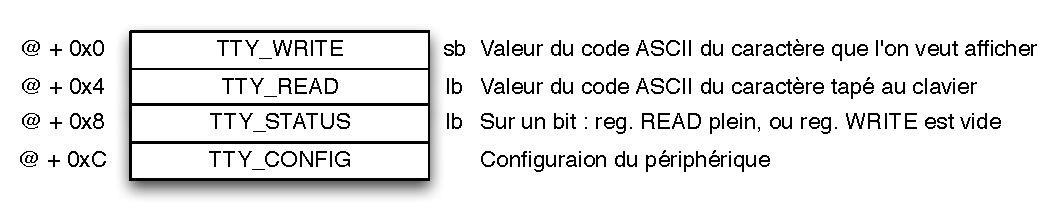
\includegraphics[scale=.75]{diagrammes/TTY}
	\caption{Le segment associé au contrôleur TTY (0x9000 0000)}
\end{figure}

\begin{rem*}
	Il y a autant de segments TTY dans l'espace adressable qu'il n'y a de périphériques TTY. Par exemple, s'i y a 3 périphériques TTY, il y aura alors 3 segments TTY correspondant à 12 registres utilisés (soit un encombrement de $3\times 12=48$ octets). 
\end{rem*}

Le programme utilisateur doit utiliser des appels systèmes pour accéder au TTY puisque le segment TTY se trouve dans la zone kernel (superviseur) de l'espace adressable. Puisque le contrôle des périphériques est exclusivement géré par l'OS, il faut impérativement passer par lui au travers d'un appel système (\lstinline!syscall!)

\subsection*{Transmission de la réponse} % (fold)
Le bus système va se charger de transmettre la réponse du périphérique cible vers le périphérique maître qui a initié la transaction.

\section{A propos des accès mémoire} % (fold)

A chaque exécution d'une instruction, le processeur doit lire en mémoire le code de l'instruction suivante. Par ailleurs, il y a différents types d'accès mémoire :\begin{itemize}
	\item Lecture de données (\lstinline!lw!);
	\item Ecriture de données (\lstinline!sw!).
\end{itemize}

Dans un programme, on trouve une moyenne de :\begin{itemize}
	\item 20\% : lecture de données (\lstinline!lw!);
	\item 10\% : écriture de données en mémoire (\lstinline!sw!);
	\item 40\% : opérations entre registres (eg. \lstinline!add!);
	\item 30\% : branchements (eg. \lstinline!jump!).
\end{itemize}

De ce fait, pour 100 instructions, on a :\begin{itemize}
	\item 120 lectures en mémoire ;
	\item 10 écritures en mémoire.
\end{itemize}

\begin{rem*}
	De plus, une écriture est non bloquante pour un programme, alors que pour une lecture, le processeur est bloqué tant que la valeur n'a pas été lue.
\end{rem*}

\chapter{Mémoires caches} % (fold)

\begin{figure}[!h]
	\center
	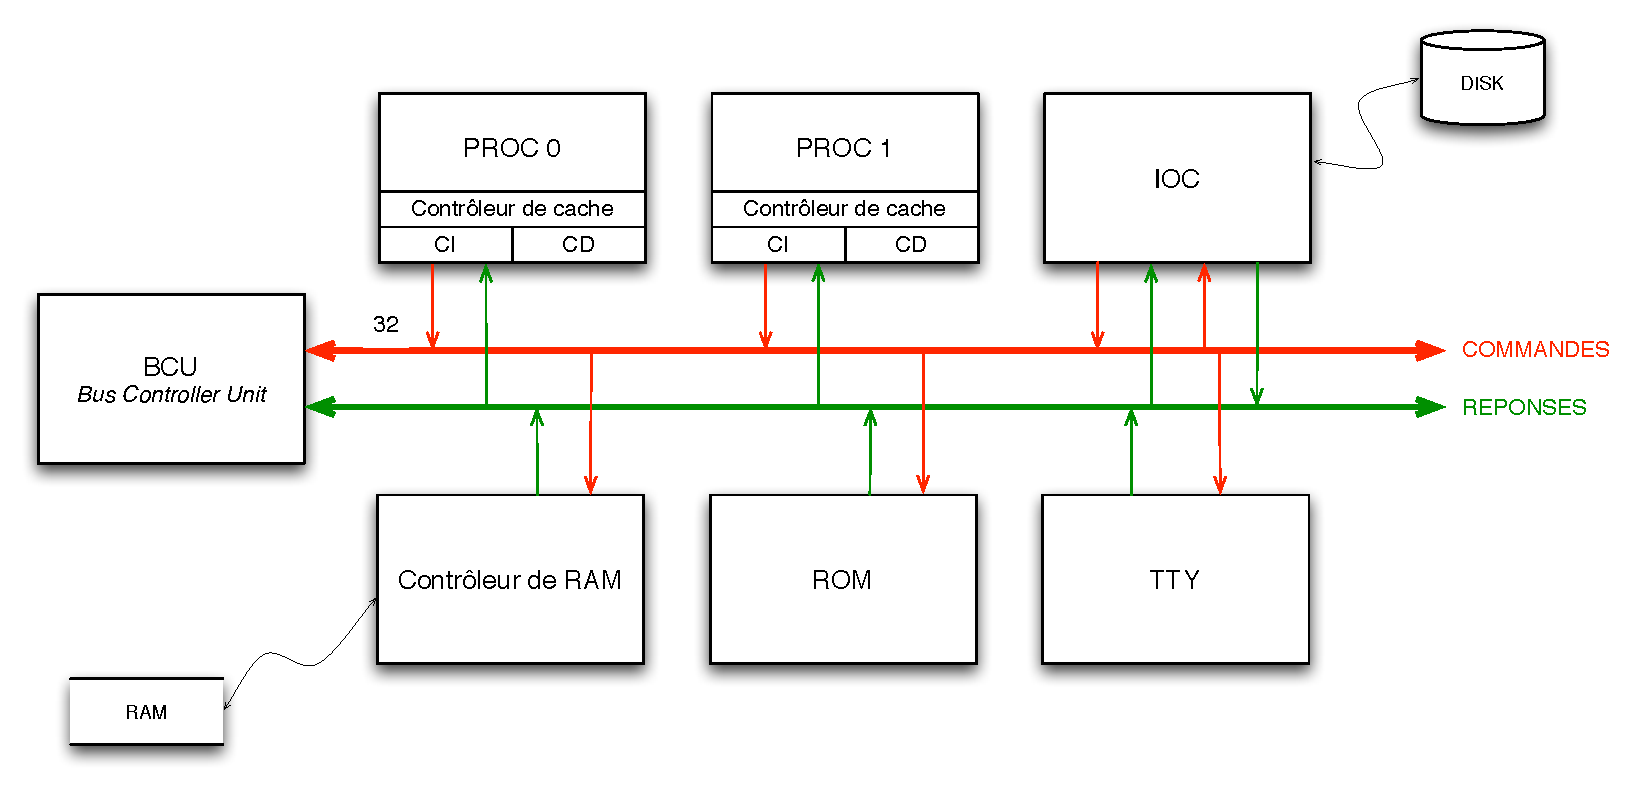
\includegraphics[scale=.5]{diagrammes/bus3}
	\caption{Composition matérielle d'un ordinateur}
\end{figure}

\section{Introduction} % (fold)

\begin{def*}[Cycle]
	Période entre deux fronts montants du signal périodique envoyé (eg. un processeur 25 MHz aura un cycle de $\nicefrac{1}{25\,000\,000}$ seconde).
	
	Le signal est distribué à tous les composants matériels $\Rightarrow$ même référence de temps entre tous ces composants.
\end{def*}

\begin{obj*}
	Eviter au processeur de passer par le bus et le BCU pour accéder à la mémoire RAM.

	Les mémoires caches doivent être très rapide pour répondre aux requêtes de lecture.
	\begin{itemize}
		\item Le temps de cycle du cache doit être égal au temps de cycle du processeur (ie. le cache doit répondre en 1 cycle) ;
		\item Cependant la capacité stockage du cache est très faible.
	\end{itemize}
\end{obj*}

Caches de premier niveau :\begin{itemize}
	\item Cache d'\textbf{instruction} (CI) : mémoire spécifique contenant des instructions ;
	\item Cache de \textbf{données} (CD) : mémoire spécifique contenant des données.
\end{itemize}

\vspace{10pt}

Il existe donc deux types de mémoire :\begin{itemize}
	\item La \textbf{mémoire dynamique} -- DRAM qui a une grande capacité de stockage\\
	L'accès à celle-ci est lent (au moins 100 fois plus lent que le cycle du processeur).
	\[
		\textrm{1 bit} \equiv \textrm{1 transistor}
	\]
	\item \textbf{Mémoire statique} -- SDRAM : très rapide (calée sur le cycle du processeur).\\
	Il y a cependant une faible capacité de stockage.
	\[
		\textrm{1 bit}\equiv\textrm{6 transistors}
	\]
\end{itemize}

\vspace{10pt}

Une mémoire cache contient des copies des informations présentes dans la mémoire principale :\begin{itemize}
	\item CI : copie d'extraits du segment \lstinline!.code! de la mémoire DRAM;
	\item CD : copie d'extraits du segment \lstinline!.data! et \lstinline!.stack! de la mémoire principale.
\end{itemize}

\section{Comment faire en sorte de minimiser le taux de MISS ?} % (fold)

\begin{def*}[Taux de MISS]
	Défini par la quotient :
	\[
		\frac{\textrm{nombre de requêtes processeur qui sont des échecs}}{\textrm{nombre total de requêtes du processeur}}
	\]
\end{def*}

\begin{def*}[Coût de MISS]
	Nombre de cycles mémoire pour réalimenter le cache. C'est le nombre de cycles pendant lesquels le processeur est gelé.
\end{def*}

La technique de cache est efficace grâce au principe de localité.

\subsection*{La localité spatiale} % (fold)

Si le processeur émet une requête à l'adresse $x$, les requêtes suivantes ont une forte probabilité de voir des adresses proches de $x$ (eg. \lstinline!PC!, \lstinline!PC+4!, \lstinline!PC+8!, \dots).

Les éléments concernés sont :\begin{itemize}
	\item Les instructions sont rangées à des adresses voisines;
	\item Les tableaux données rangées à des adresses consécutives.
\end{itemize}

\subsection*{La localité temporelle} % (fold)

Si le processeur émet une requête à l'adresse $x$ au cycle $n$, il arrive très souvent qu'une autre requête soit effectuée à le même adresse $x$, au cours des cycles suivant le cycle $n$.

Les éléments concernés sont :\begin{itemize}
	\item Les programmes contiennent des boucles (cache d'instructions);
	\item Les programmes contiennent des compteurs (cache de données).
\end{itemize}

\section{Comment exprimer le voisinage ?} % (fold)

\begin{def*}[Ligne de cache]
	Découpage / tranche de l'espace adressable.
	
	Attention. Une ligne de cache n'est pas une information actuellement stockée dans le cache.
\end{def*}

Tous les octets d'une même ligne de cache sont voisins entre eux. 

\begin{def*}[Voisinage]
	Soit un octet rangé à l'adresse $x$.\\
	Le voisinage de $x$ est l'ensemble des octets qui appartiennent à la même ligne que $x$.
\end{def*}

En cas de MISS, sur une requête à l'adresse $x$, le contrôleur de cache va ramener dans le cache une ligne complète contenant l'adresse $x$.\\
$\Rightarrow$ Utilisation de la localité \textbf{spatiale}.

Pour exploiter la localité \textbf{temporelle}, le contrôleur de cache conserve dans le cache le plus longtemps possible les informations récupérées dans la mémoire.

\begin{figure}[!h]
	\center
	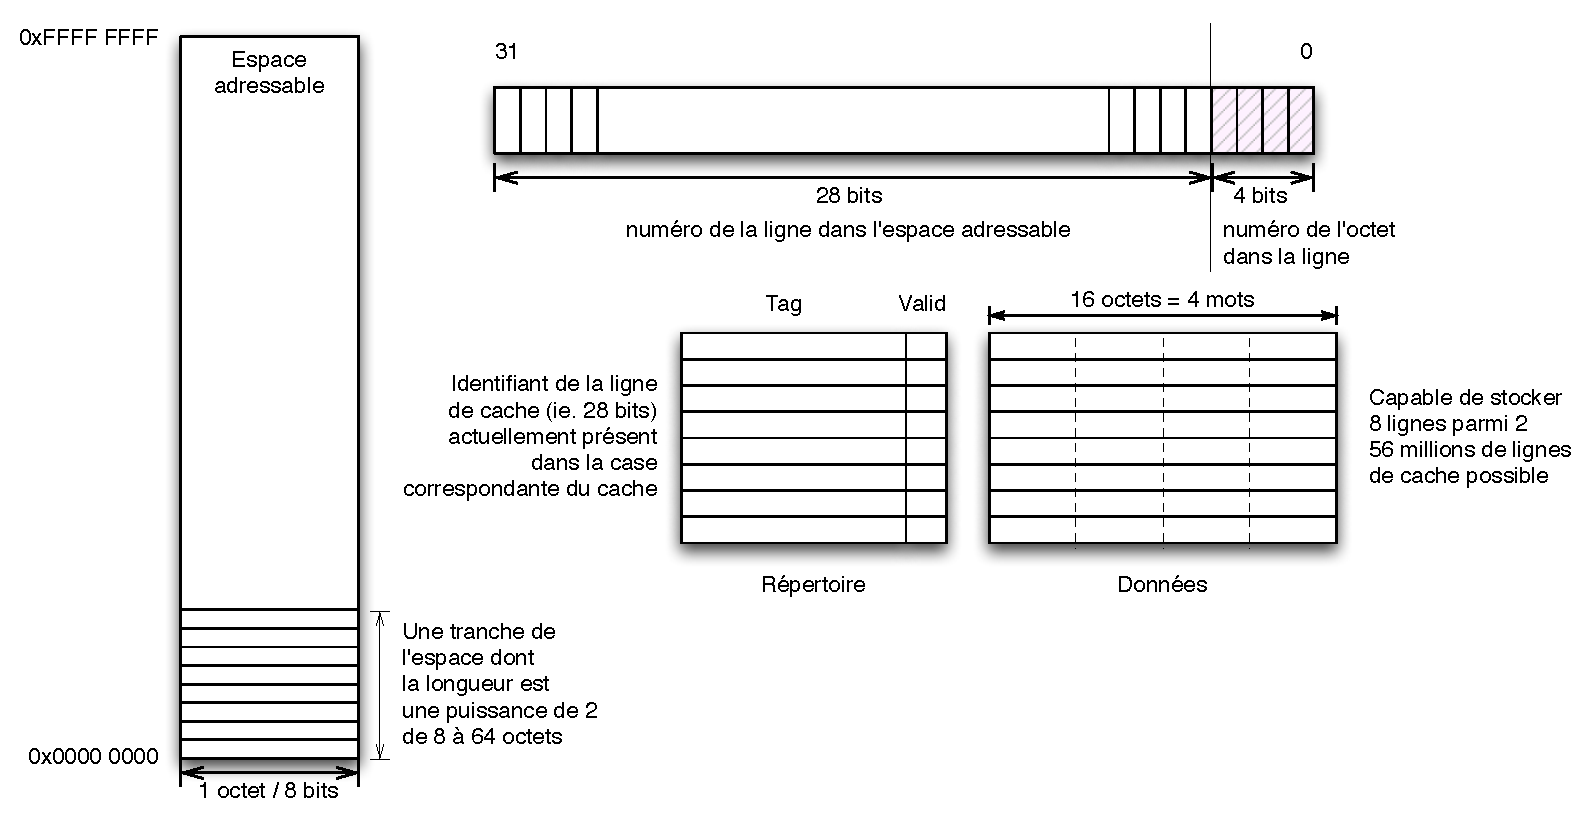
\includegraphics[scale=.65]{diagrammes/cache}
	\caption{Caches à correspondance directe}
\end{figure}

\begin{description}
	\item[Stratégie 1] \textbf{Cache associatif} (\emph{associative})\\
  	$\Rightarrow$ N'importe quelle ligne peut être rangée dans n'importe quelle case\\
	Les huit cases sont équivalentes entre elles. Le processeur cherche à savoir si la ligne est dans le cache $\rightarrow$ regarder dans chaque case si elle est présente (séquentiellement) : il y a \lstinline!nb_cases! comparaisons.
  
	\item[Stratégie 2] \textbf{Cache à correspondance directe} (\emph{direct mapping})\\
	$\Rightarrow$ Une ligne de cache ne peut être rangée que dans une seule case.\\
	Les cases ne sont plus équivalentes entre elles. Toutes les lignes de cache d'une même famille sont en compétition pour la même case.\\
	$\Rightarrow$ Retrouver une ligne de cache à partir de son adresse est beaucoup plus rapide car on accède directement à la seule case possible.
\end{description}
\clearpage
\section{Comment faire cette partition ?} % (fold)

\begin{figure}[!h]
	\center
	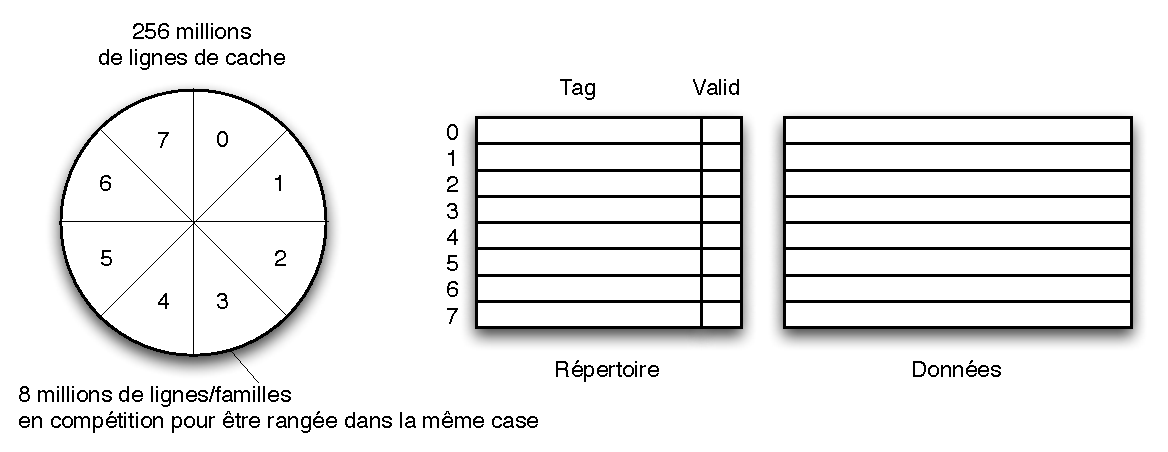
\includegraphics[scale=.65]{diagrammes/caches-familles}
	\caption{Cache à correspondance directe}
\end{figure}

Si deux lignes voisines sont dans la même famille, elles seraient en compétition pour la même case de cache $\Rightarrow$ Le principe de localité n'est pas respecté.

\begin{figure}[!h]
	\center
	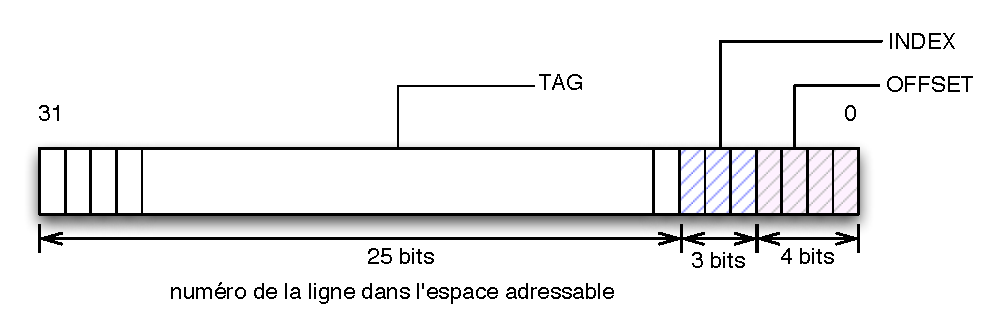
\includegraphics[scale=.65]{diagrammes/adresse-cache}
	\caption{Adresse dans le cache}
\end{figure}

Les champs de l'adresse :\begin{itemize}
	\item OFFSET $\equiv$ numéro de mot dans la case du cache : $\log_2(\textrm{taille ligne})$ ;
	\item INDEX $\equiv$ numéro de la famille $\equiv$ numéro de case de cache : $\log_2(\nicefrac{\textrm{taille cache}}{\textrm{taille ligne}})$ ;
	\item TAG $\equiv$ numéro identifiant une ligne de cache dans la famille : $32 - (\textrm{OFFSET} + \textrm{INDEX})$.
\end{itemize}

\begin{figure}[!h]
	\center
	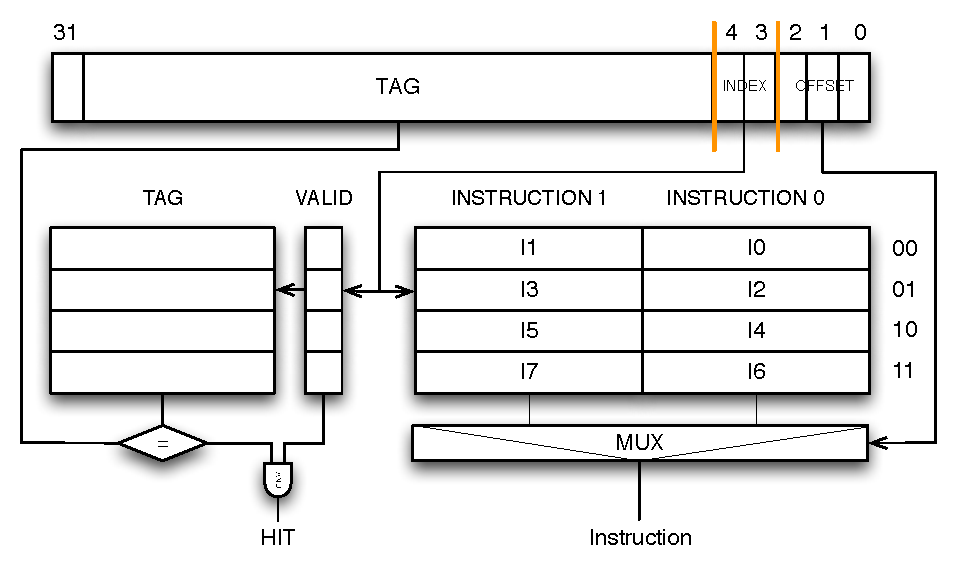
\includegraphics[scale=.65]{diagrammes/cache2}
	\caption{Principe résumé d'un cache}
\end{figure}

\section{Le problème des écritures} % (fold)
Il n'y a pas de symétries entre les lectures et les écritures.\\
But du cache : accélérer les lectures (\lstinline!lw!).

Les caches contiennent des \emph{copies} de la mémoire principale.\\
$\Rightarrow$ Problème de cohérence entre le cache et la mémoire

Synchronisation producteur / consommateur.

\begin{figure}[!h]
	\center
	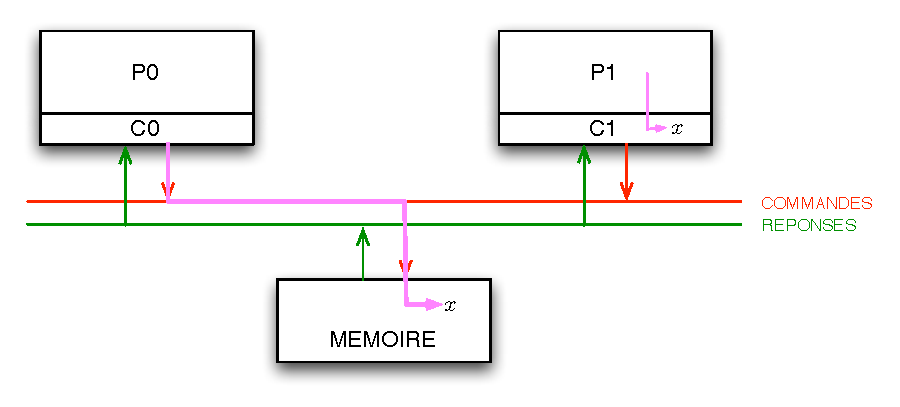
\includegraphics[scale=.5]{diagrammes/ecriture-caches}
	\caption{Ecriture dans la mémoire}
\end{figure}

\begin{description}
	\item [WRITE-THROUGH] Une écriture est effectuée immédiatement vers la
	  mémoire (avec mise à jour de la copie locale\dots si elle existe).
	  \item[WRITE-BACK] Une écriture est effectuée dans le cache local, et la
	  mémoire n'est pas mise à jour plus tard, que en cas d'évincement.
	  \item[Contradictions] \hfill \begin{itemize}
			\item Quand le processeur fait un \lstinline!sw!, cette instruction n'est pas bloquante;
			\item Quand le contrôleur de cache fait une écriture, il attend un acquittement. Le contrôleur de cache contient un tampon d'écritures postées (file FIFO du cache de données \emph{Write Buffer})
		\end{itemize}
		\begin{rem*}
			L'utilité de cette file d'attente matérielle est double: \begin{itemize}
				\item Le processeur n'est pas bloqué;
				\item On peut espérer fabriquer des rafales d'écriture, et donc optimiser  l'utilisation du bus.
			\end{itemize}
		\end{rem*}
\end{description}

\section{Influence des caches sur les performances} % (fold)

\begin{def*}[CPI -- \emph{Cycle Per Instruction}]
	Le CPI (\emph{Clock cycles Per Instruction} ou \emph{Clocks per Instruction})est utilisé pour décrire la performance d'un processeur. Il correspond au nombre de cycles moyen pendant lesquels une instruction est exécutée.
	
	L'objectif est de minimiser ce taux en le rapprochant de 1. Dans le cas où le CPI est égal à 1 pour un unique processeur, il y a un cycle mémoire parfait (ie. taux HIT = 100\% et taux MISS = 0\%).
\end{def*}

Dans une architecture RISC pipeline, chaque instruction est découpée en 5 cycles : \begin{enumerate}
	\item \emph{Instruction Fetch cycle} (IF) : accès au cache pour récupérer l'instruction ;
	\item \emph{Instruction decode} / \emph{Register fetch cycle} (ID) : décodage de l'instruction ;
	\item \emph{Execution} / \emph{Effective address cycle} (EX) : exécution de l'instruction ;
	\item \emph{Memory access} (MEM) : cherche en mémoire le contenu se trouvant à l'adresse donnée ;
	\item \emph{Write-back cycle} (WB) : transmission du résultat en mémoire dans un registre.
\end{enumerate}

Chaque étape requière un cycle d'horloge et une instruction va suivre séquentiellement chaque étape.

	Dans une architecture sans pipeline, une nouvelle instruction est récupérée (IF) dans la première étape seulement une fois que l'instruction précédente ait fini l'étape 5 (WB).
	
	Dans une architecture avec pipeline, le CPI peut être amélioré en utilisant l'\emph{instruction level parallelism} (ILP). Ainsi, une nouvelle instruction est récupérée (IF) à chaque cycle. Dans le cas où  il y aurait 5 instructions dans 5 étapes de pipeline différentes (une instruction par étape), une instruction différente complèterait l'étape 5 (WB) pour chaque cycle d'horloge. De ce fait, le CPI est égal à 1 pour ce processeur.

\begin{def*}[IPC -- \emph{Instruction Per Cycle}]
	Le CPI est l'inverse de l'IPC (\emph{Instruction Per Cycle}) égal au nombre moyen d'instructions exécutées par cycle d'horloge.
\end{def*}

\begin{def*}[IPS -- \emph{Instruction Per Second}]
	Le nombre d'instructions par seconde IPS (\emph{Instruction Per Second}) est égal à : $CPI \times clock\_speed$ où $clock\_speed$ est la fréquence du processeur considéré calculée en Hertz (Hz) ou en cycles par seconde.
\end{def*}

\begin{figure}[!h]
	\center
	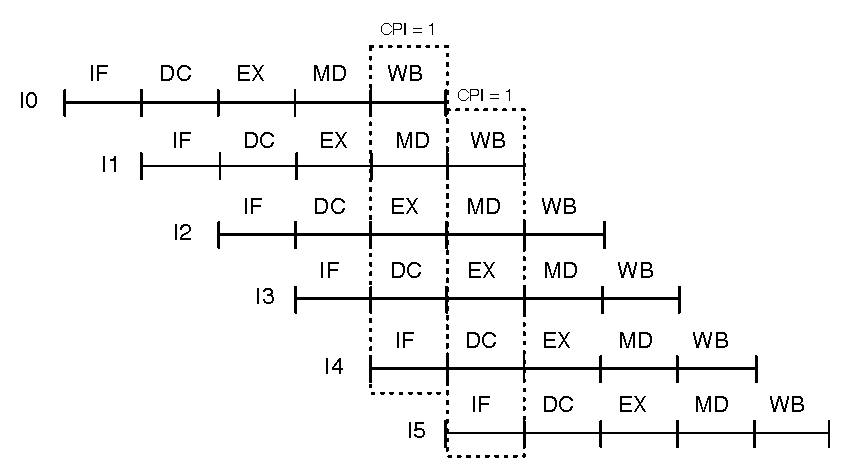
\includegraphics[scale=.65]{diagrammes/pipeline}
	\caption{Minimisation du CPI}
\end{figure}


\chapter{Retour sur EXCEPTIONS / INTERRUPTIONS / TRAPPES}

Plusieurs programmes peuvent s'exécuter simultanément sur une même machine. Le système d'exploitation gère alors les accès matériel.

Le système d'exploitation (GIET) est un logiciel qui est activé dans trois cas. Son \textbf{point d'entrée} se situe à l'adresse 0x8000 0180.

\section{Appel système / Trappe} % (fold)

Exécution (par un programme utilisateur) de l'instruction \lstinline!syscall! :\\
(\$2$\leftarrow$ code de l'appel / \$4 à \$7 $\leftarrow$ arguments).

Ce sont des appels effectués par un programme utilisateur vers le système d'exploitation pour un service (eg. écriture sur un terminal , écriture sur un disque, \dots).

Le gestionnaire d'appels systèmes du GIET doit effectuer :
\begin{itemize}
	\item EPC $\leftarrow$ PC
	\item PC $\leftarrow$ 0x80000180
	\item SR $\leftarrow$ mode kernel, IT masquées
	\item CR $\leftarrow$ \lstinline!system call handler address! (saut à cette adresse)
	\item Numéro de service demandé (dans le registre \$2)
	\item Valeur des arguments (dans les registres \$4 à \$7)
	\item Appel de la fonction système requise
	\item EPC $\leftarrow$ adresse de retour (instruction \lstinline!eret!)
\end{itemize}

\section{Exception} % (fold)

Exécution (par un programme utilisateur) d'une instruction illégale~:\vspace{-10pt} \begin{multicols}{2}
\begin{itemize}
		\item ADEL -- lecture illégale
		\item ADES -- écriture illégale
		\item DBE -- Bus erreur données
		\item IBE -- Bus erreur instruction
		\item OVF -- overflow arithmétique
		\item RI -- codop indéfini !
		\item CPU -- tentative d'exécution \lstinline!mfc0! ou \lstinline!mtc0!
	\end{itemize}
\end{multicols}
\vspace{-10pt}

Le gestionnaire d'exceptions doit déterminer le type de l'exception et afficher un message permettant au programmeur de localiser et de corriger l'erreur.

\begin{rem*}\hfill
	\begin{itemize}
	\item Les codes du type d'exception sont écrits par le matériel dans le registre CR
	\item L'adresse de l'instruction fautive est écrite dans EPC
	\item BAR $\leftarrow$ adresse fautive
	\item SR $\leftarrow$ Mode Kernel (UM = 0) -- IT (interruption) masquées (IE = 0)
	\item PC $\leftarrow$ 0x80000180~: point d'entrée dans le système.
	\end{itemize}
\end{rem*}

\section{Interruptions / communication avec les périphériques} % (fold)

Deux entités communiquent :\begin{itemize}
	\item Le ``périphérique'' -- l'utilisateur ;
	\item Le système d'exploitation (et non le programme qui s'exécute sur le processeur).
\end{itemize}

Les interruptions provenant de périphériques sont imprévisibles du point de vue du programme en cours d'exécution et peuvent donc survenir à tout instant.

Si elle n'est pas masquée, l'activation d'interruption déclenche l'exécution d'une routine spécifique (ISR) permettant au périphérique de ``voler'' des cycles au processeur. Le programme interrompu reprend ensuite son exécution normale. 

Le gestionnaire d'interruptions doit déterminer la source de l'interruption pour activer la bonne ISR en interrogeant le composant ICU. 

\subsection{Communication avec les périphériques} % (fold)

\begin{figure}[!h]
	\center
	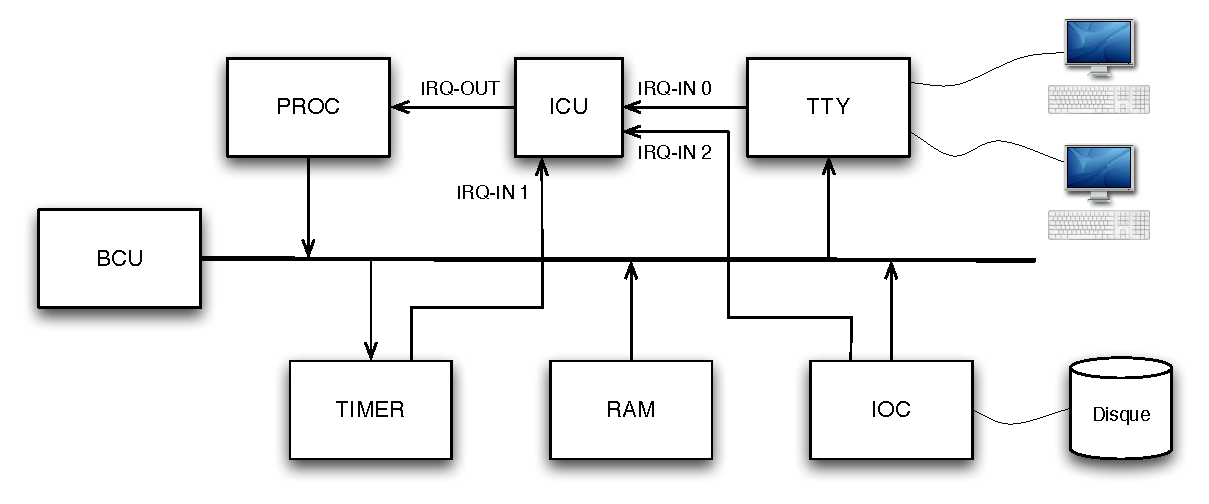
\includegraphics[scale=.5]{diagrammes/ICU-bus}
	\caption{Gestion des interruptions (IRQ)}
\end{figure}

Le système d'exploitation gère donc les mécanismes de contrôle. Il existe deux types de communications entre le système d'exploitation et les périphériques :\begin{itemize}
	\item \textbf{Accès en configuration} (opération d'écriture sur des registres du périphérique) ou \textbf{accès en consultation} (opération de lecture);
	\item Initiatives venant du périphérique pour signaler des évènements à l'OS (\textbf{interruptions}). 
\end{itemize}

Communication entre deux processus : suivant le modèle producteur / consommateur.

\begin{idee*}
	Le périphérique et l'OS communiquent à travers un tampon mémoire partagé ou plusieurs. Dans le cas du TTY, il est nécessaire d'avoir deux tampons : \begin{itemize}
		\item Un tampon DATA (\lstinline!TTY_WRITE!) qui contient le caractère tapé au clavier -- 1 octet en mémoire correspondant à la taille mémoire d'un caractère ASCII;
		\item Un tampon FULL (\lstinline!TTY_STATUS!) contenant un booléen (1 bit) qui indique l'état du tampon DATA :\begin{itemize}
			\item Producteur : FULL $\leftarrow$ 1 si tampon DATA rempli;
			\item Consommateur : FULL $\leftarrow$ 0 si tampon DATA lu et vidé.
		\end{itemize}
	\end{itemize}
\end{idee*}

\begin{def*}[IRQ -- \emph{Interrupt Request}]
	Une interruption (IRQ) provient d'un contrôleur / périphérique et arrive dans l'ICU (\emph{Interrupt Controllor Unit}). L'IRQ demande alors au processeur d'exécuter l'ISR (\emph{Interrupt Service Routine}) correspondante.
\end{def*}

\begin{def*}[ISR -- \emph{Interrupt Service Routine}]
	Un périphérique (TTY, Timer, \dots) souhaite effectuer une écriture en mémoire, active une interruption qui va forcer le processeur à exécuter quelques dizaines / centaines d'instructions.

	Ce code s'appelle ISR (\emph{Interrupt Service Routine}).

	Activation : il y a une ISR différente pour chaque périphérique.

	Instructions de l'ISR :\begin{itemize}
		\item Ecrit dans le registre de communication et de synchronisation;
		\item Ecrit dans le registre du périphérique permettant d'acquitter la requête d'interruption.
	\end{itemize}
\end{def*}

\begin{def*}[ICU -- \emph{Interrupt Controller Unit}]
	Ce contrôleur comporte (dans le cadre du cours) 32 lignes d'interruption en concurrence pour voler des cycles au processeur. Le composant ICU est un concentrateur d'interruptions permettant de \textbf{multiplexer} 32 interruptions IRQ-IN vers \textbf{une} interruption IRQ-OUT.
\end{def*}

\subsection{Comment le gestionnaire d'interruptions peut-il déterminer quel ISR exécuter ?} % (fold)

\paragraph{Organisation générale du GIET} % (fold)

Lors d'un appel système, d'une interruption, d'une exception, il y a un branchement à l'adresse 0x80000180 -- point d'entrée du GIET (Gestionnaire d'Interruptions, Exceptions et Trappes).

\begin{figure}[!h]
	\center
	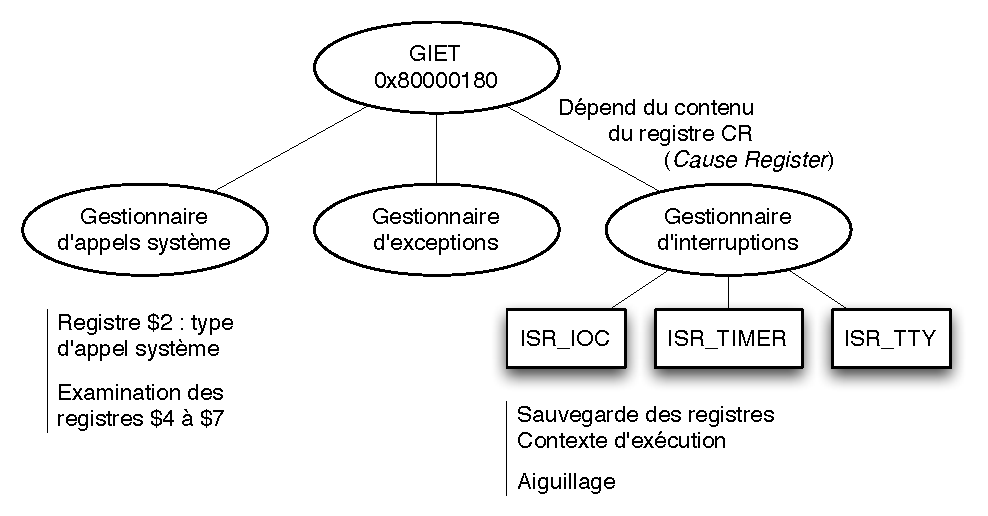
\includegraphics[scale=.5]{diagrammes/GIET}
	\caption{Organisation du GIET}
\end{figure}

Les interruptions sont vectorisées. 

\begin{def*}[Vecteur d'interruptions]
	Un tableau en mémoire dont chaque entrée est une adresse d'une ISR. C'est donc un tableau d'adresse où chaque adresse correspond à un point d'entrée d'une fonction du GIET.
\end{def*}

\begin{rem*}
	Un tableau d'adresse $\equiv$ table de sauts $\equiv$ vecteur d'interruptions
\end{rem*}

Le gestionnaire d'interruptions détermine l'index (index compris entre 0 et 31) vers lequel il va se brancher. Pour obtenir l'index en question, le gestionnaire d'interruptions interroge le composant ICU en effectuant une lecture dans son registre INDEX.

Conflit : si plusieurs IRQ-IN sont actives en même temps, l'ICU renvoie l'index le plus petit.

\begin{rem*}
	ICU (\emph{Interrupt Controller Unit}) $\equiv$ PIC (\emph{Programmable Interrupt Controller})
\end{rem*}

\begin{figure}[!h]
	\center
	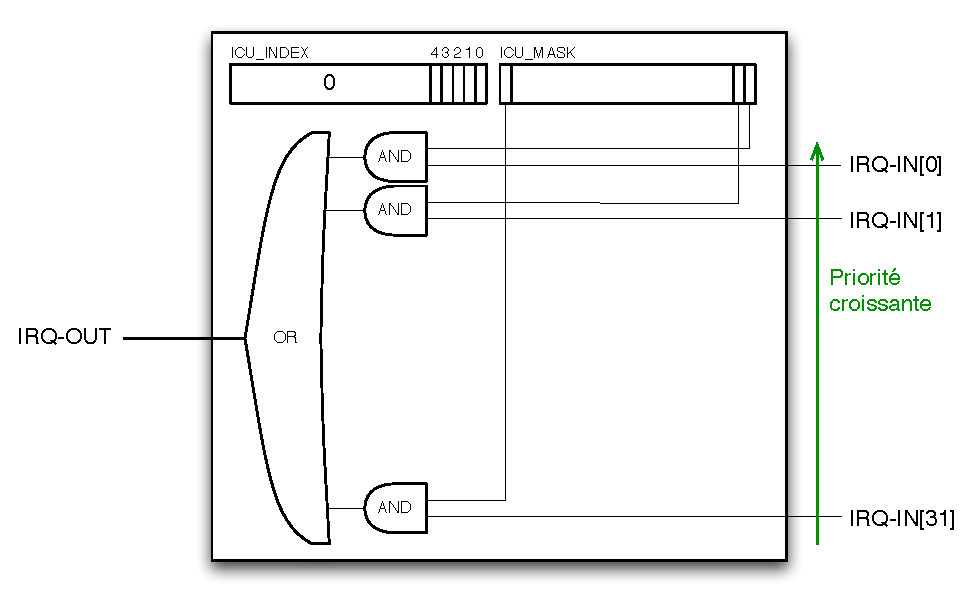
\includegraphics[scale=.5]{diagrammes/ICU}
	\caption{ICU (\emph{Interrupt Controller Unit})}
\end{figure}

Registres de l'ICU : \begin{itemize}
	\item \lstinline!ICU_MASK! : chaque bit représente la gestion d'une interruption des 32 interruptions possibles : \begin{itemize}
		\item \lstinline!ICU_MASK!$[i] = 0$ : pas d'interruption sur l'entrée $i$ (interruption masquée);
		\item \lstinline!ICU_MASK!$[i] = 1$ : interruption autorisée sur l'entrée $i$. 
	\end{itemize}
	Les interruptions ont par défaut une priorité croissante (ie. l'interruption de l'entrée 1 sera traitée avant celle de l'entrée 2).
	\item \lstinline!ICU_INDEX! : numéro de l'interruption la plus prioritaire active (registre codé sur 5 bit -- $2^5=32$).
\end{itemize}

Résumé sur les services rendus par l'ICU :\begin{enumerate}
	\item OU logique entre toutes les entrées IRQ-IN($i$);
	\item Encodeur de priorité;
	\item Masque sélectif M[$i$] des 32 IRQ-IN[$i$] (ce masque tient sur un mot de 32 bits).
\end{enumerate}

\begin{idee*}
	On augmente la complexité du matériel en ayant plusieurs IRQ-OUT.
	
	Si on réplique 8 fois le matériel de l'ICU, on aura les 32 mêmes entrées IRQ-IN, et 8 sorties IRQ-OUT.
	
	On va avoir 8 IR-OUT[$j$] et on peut donc ``router'' chaque IRQ-IN[$i$] vers n'importe quelle sortie IRQ-OUT[$j$].
	
	D'où PIC : \emph{\textbf{Programmable} Interrupt Controller}
\end{idee*}

\begin{rem*}
	L'OS doit configurer les registres de masque de l'ICU et doit initialiser le vecteur d'interruptions (généralement dans le code de BOOT).
	
	Le code des ISR ne fait pas partie de l'OS, mais il s'exécute en général en mode superviseur.
\end{rem*}

\section{A propos de l'appel au GIET} % (fold)

\begin{wrapfigure}{r}{0.37\textwidth}
	\vspace{-30pt}
	\center
	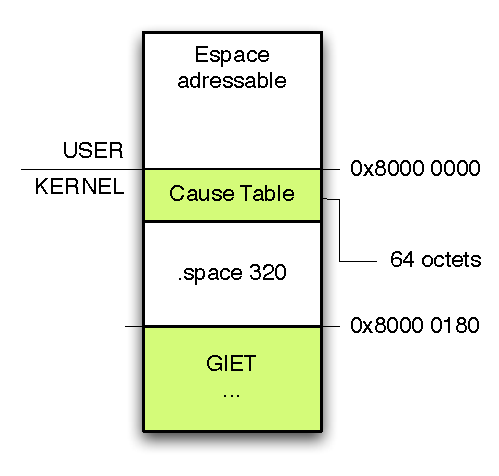
\includegraphics[scale=.5]{diagrammes/cause-table}
	\vspace{-10pt}
\end{wrapfigure}

La cause de l'activation du GIET est située dans le registre CR (\emph{Cause Register}). Le GIET parcourt alors la table \emph{Cause table}, une table de sauts contenant les adresses des fonctions à appeler suivant la valeur du registre CR. Cette table est située à l'adresse 0x8000 0000 et contient 16 entrées (taille : $16\times 4=64$ octets).

Lorsque le processeur se branche à la première instruction du GIET, les interruptions sont automatiquement masquées par le matériel :\begin{itemize}
	\item Si la cause du branchement est une exception, il y a alors un traitement prioritaire de l'exception et on ne souhaite pas être interrompu ;
	\item Si la cause du branchement est une interruption, il faut pouvoir exécuter le code du GIET sans reboucler sur cette adresse. En effet, à chaque cycle, le processeur examine le contenu du registre \lstinline!IRQ_INDEX! ;
	\item Si la cause du branchement est un appel système, alors le GIET doit décider lui-même d'être interrompu ou non. 
\end{itemize}

\vspace{30pt}

\subsection{Le registre d'état SR (\emph{Status Register})} % (fold)

\begin{figure}[!h]
	\center
	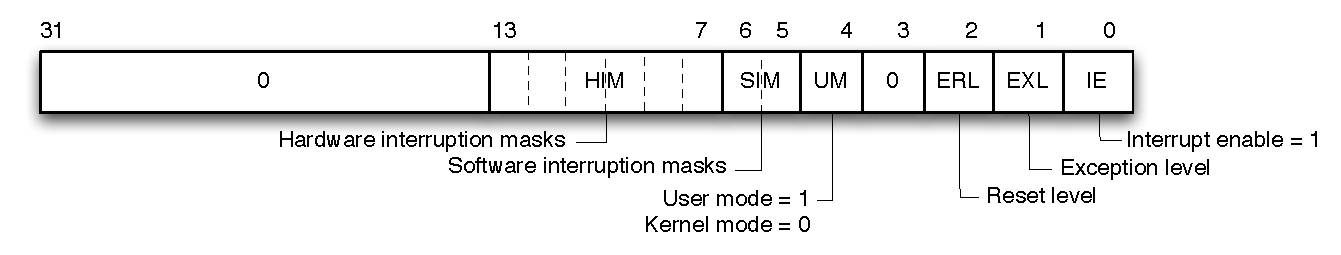
\includegraphics[scale=.65]{diagrammes/SR}
	\caption{SR (\emph{Status Register})}
\end{figure}

\begin{itemize}
	\item Le processeur a le droit d’accéder aux ressources protégées (registres du CP0, et adresses mémoires supérieures à 0x7FFFFFFF) si et seulement si le bit UM vaut 0, ou si l’un des deux bits ERL et EXL vaut 1 ;
	\item Les interruptions sont autorisées si et seulement si le bit IE vaut 1, et si les deux bits ERL et EXL valent 00, et si le bit correspondant de IM vaut 1 ;
	\item Les trois types d’événements qui déclenchent le branchement au GIET (interruptions, exceptions et appels système) forcent le bit EXL à 1, ce qui masque les interruptions et autorise l’accès aux ressources protégées ;
	\item L’activation du signal RESET qui force le branchement au Boot-Loader force le bit ERL à 1, ce qui masque les interruptions et autorise l’accès aux ressources protégées ;
	\item L’instruction \lstinline!eret! force le bit EXL à 0.
\end{itemize}

Lors de l’activation du RESET, SR contient donc la valeur 0x0004. Pour exécuter un programme utilisateur en mode protégé, avec interruptions activées, il doit contenir la valeur 0xFF11. Le code de boot doit écrire la valeur 0xFF13 dans SR et l’adresse du programme utilisateur dans EPC avant d’appeler l’instruction \lstinline!eret!.

\subsection{Le registre de cause CR (\emph{Cause Register})} % (fold)

\begin{figure}[!h]
	\center
	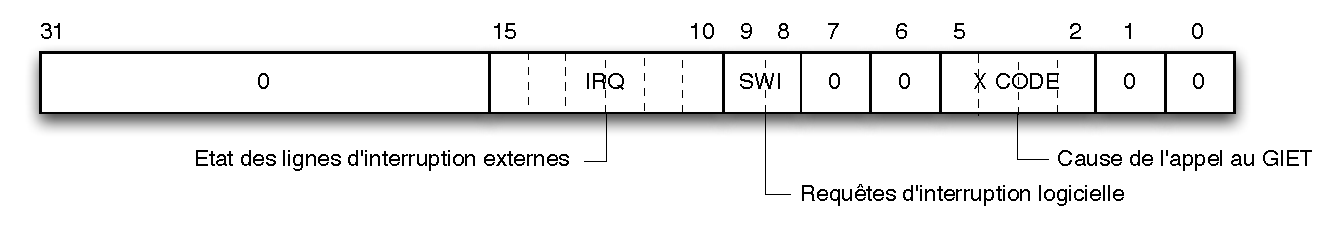
\includegraphics[scale=.65]{diagrammes/CR}
	\caption{CR (\emph{Cause Register})}
\end{figure}

Le registre CR contient trois champs. Les 4 bits du champs XCODE(3:0) définissent la cause de l'appel au GIET. Les 6 bits du champs IRQ(5:0) représentent l'état des lignes d'interruption externes au moment de l'appel au GIET. Les 2 bits SWI(1:0) représentent les requêtes d'interruption logicielle.


\chapter{Périphériques} % (fold)

Le pilote de périphérique contient deux parties :\begin{itemize}
	\item Un code de ``configuration'' : permet au logiciel (OS) de lire / écrire dans les registres internes au périphérique. A l'initiative de l'OS. Ce code se trouve dans le fichier \lstinline!drivers.c! ;
	\item Le(s) code(s) de(s) ISR (\emph{Interrupt Service Routine}) permettant au périphérique de communiquer avec l'OS. A l'initiative du périphérique. Ce code se trouve dans le fichier \lstinline!isr.s!. 
\end{itemize}

\begin{figure}[!h]
	\center
	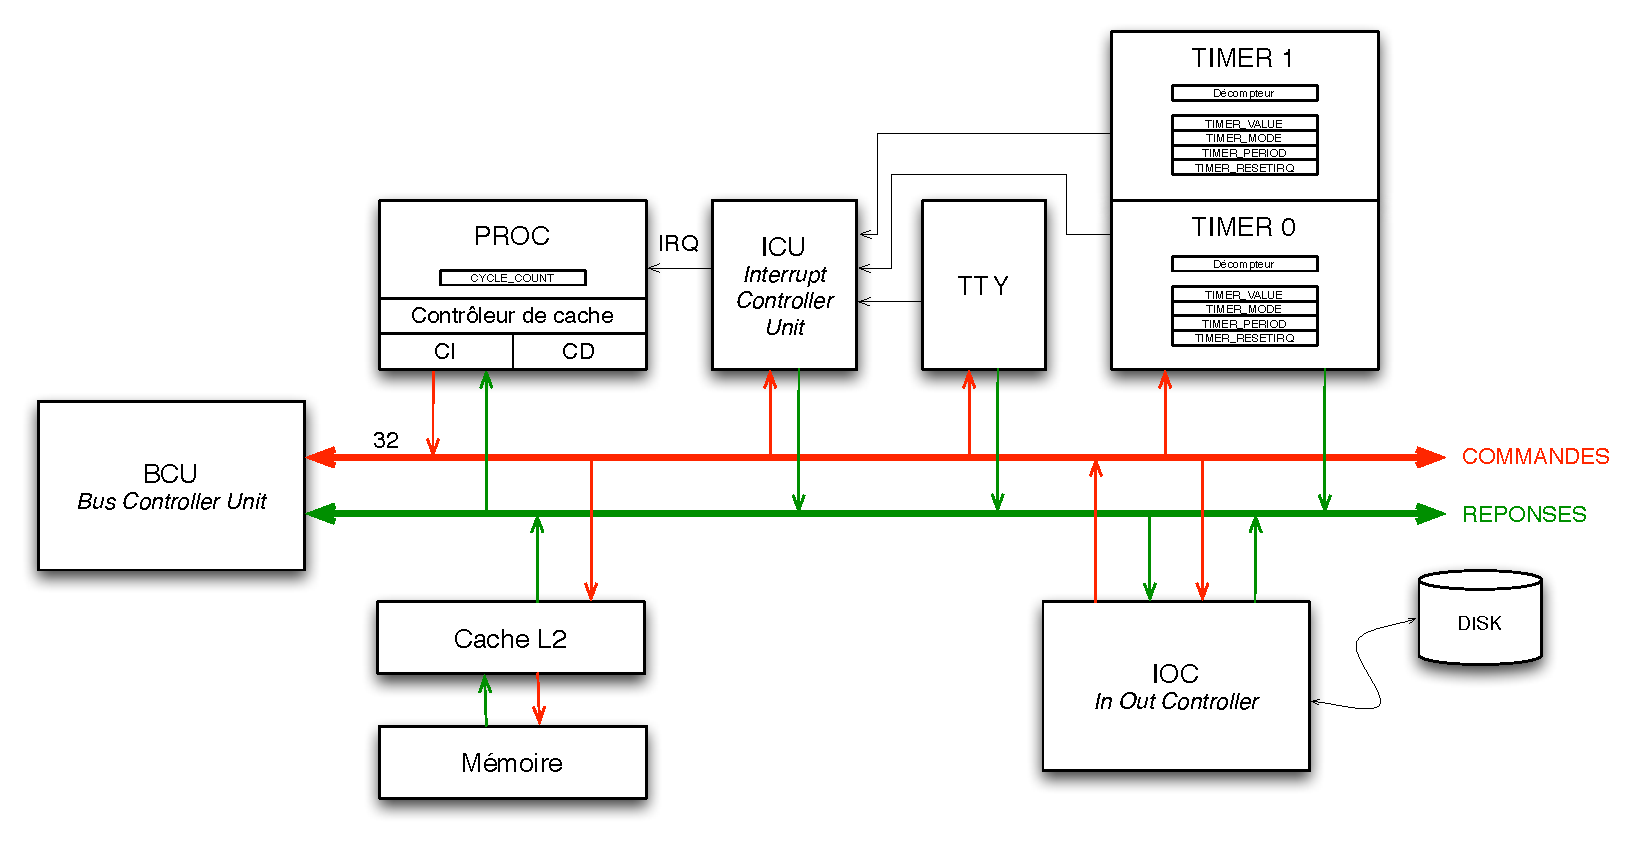
\includegraphics[scale=.63]{diagrammes/timer}
	\caption{Quelques périphériques}
\end{figure}

Les périphériques sont de deux sortes :\begin{itemize}
	\item Périphérique ``simple'' : pouvant recevoir des commandes de lecture / écritures, mais ne peuvent pas eux-mêmes lire ou écrire dans l'espace adressable (eg. TIMER, ICU, contrôleur TTY\dots) ;
	\item Périphériques DMA (\emph{Direct Memory Access}) : a le droit de lire / écrire d'eux-même dans l'espace adressable.
\end{itemize}

\section{Un périphérique simple : le TIMER} % (fold)

Il existe plusieurs types de TIMER :\begin{itemize}
	\item Le compteur de cycles (privé) dans chaque processeur -- registre protégé \lstinline!CYCLE_COUNT!;
	\item Le périphérique externe utilisable par le logiciel (OS) pour générer des interruptions périodiques.
\end{itemize}

\begin{wrapfigure}{r}{0.37\textwidth}
	\center
	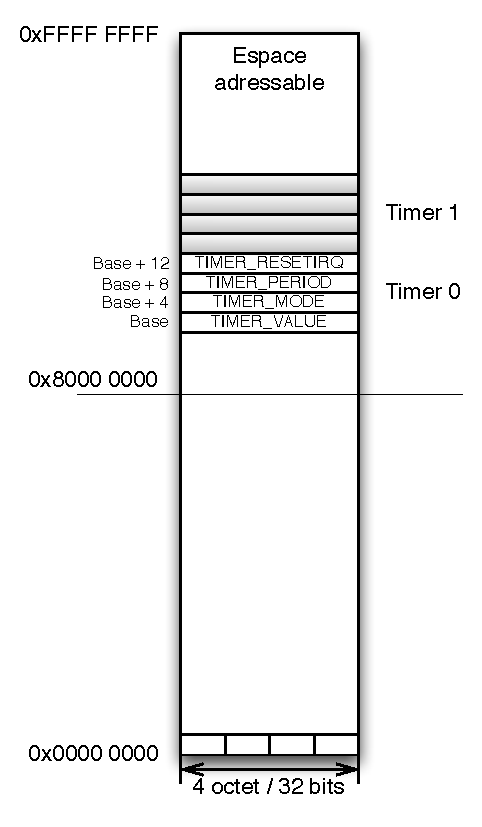
\includegraphics[scale=.5]{diagrammes/timer_addresses}
	\vspace{-10pt}
	\caption{Les registres adressables des timers}
	\vspace{-35pt}
\end{wrapfigure}

Les registres adressables du TIMER :\begin{itemize}
	\item Registre \lstinline!TIMER_VALUE! (Base) : compteur de cycles;
	\item Registre \lstinline!TIMER_MODE! (Base + 4) : configuration -- contient un CODOP écrit par le logiciel sur 2 bits :
	\begin{itemize}
		\item incrémenter (1 bit);
		\item masquer des interruptions (1 bit).
	\end{itemize}
	\item Registre \lstinline!TIMER_PERIOD! (Base + 8) : Valeur de la période où l'OS lève des interruptions (généralement égale à $100\, 000$ ou $1\, 000\, 000$);
	\item Registre \lstinline!RESETIRQ! (Base + 12) : acquittement -- fin du traitement de l'interruption.
\end{itemize}

Le registre caché \lstinline!DECOMPTEUR! du TIMER n'est pas adressable. C'est un décompteur périodique se basant sur la période définie par l'OS dans le registre \lstinline!TIMER_PERIOD! interne au TIMER.

\vspace{10pt}

Le périphérique TIMER peut contenir plusieurs timers : chaque timer individuel contient les 5 registres physiques et correspond à 4 registres adressables dans l'espace adressable.

\section{Un périphérique ``BLOCS'' : IOC (\emph{In Out Controller})} % (fold)

On parle de périphérique ``orienté blocs'' lorsque l'on doit désigner des objets dans un autre espace de stockage (généralement beaucoup plus grand\dots et beaucoup plus \textbf{lent}).

\begin{figure}[!h]
	\center
	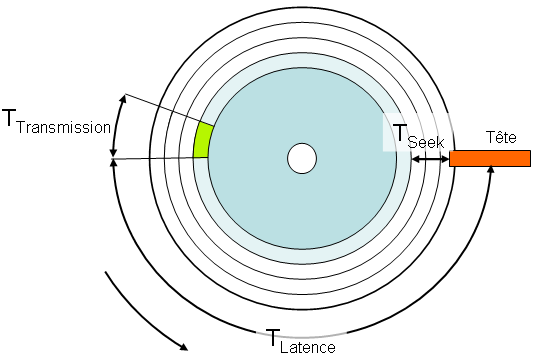
\includegraphics[scale=.5]{diagrammes/Dd4}
	\caption{Disque dur}
\end{figure}

Hiérarchie de stockage

\begin{tabularx}{\linewidth}{Xcc}
\toprule 
Espace de stockage & Taille & Temps d'accès\tabularnewline
\midrule
\midrule 
32 registres généraux & $32\times4=128$ octets & < 1 cycle\tabularnewline
\midrule 
Caches L1 & 4 Ko & 1 cycle\tabularnewline
\midrule 
Cache L2 & 4 Mo & 20 cycles\tabularnewline
\midrule 
Mémoire externe (RAM, ROM) & 2 Go & 400 cycles\tabularnewline
\midrule 
Disque & 200 Go & $100\,000$ à $1\,000\,000$ cycles\tabularnewline
\bottomrule
\end{tabularx}

\begin{def*}[Bloc]
	On appelle ``bloc'' un ensemble d'octets (varie entre 512 octets et 4096 octets) qui vont être rangés à des adresses consécutives en mémoire.
\end{def*}

\begin{def*}[Secteur]
	L'emplacement sur le disque permettant de stocker un bloc s'appelle un secteur. La taille typique d'un secteur est de 512 octet.
\end{def*}

Pour désigner un bloc dans l'``espace disque'', le logiciel utilise un ``numéro de bloc''.

Pour désigner un bloc à transférer, il faut deux instructions :\begin{itemize}
	\item Nom de fichier -- chemin / nom ;
	\item Un numéro de bloc dans un fichier.
\end{itemize}

\vspace{7pt}

Transférer un (ou plusieurs) blocs depuis le disque vers la mémoire :\begin{itemize}
	\item Nom de fichier : appel système \lstinline!ioc_read()! renvoie un descripteur de fichier (\lstinline!FILE *!) ;
	\item Désigner le premier bloc et le nombre de blocs à transférer ;
	\item Désigner l'adresse de base du tampon mémoire cible.
\end{itemize}

\vspace{7pt}

Deux appels systèmes du GIET :
\vspace{-5pt}\begin{lstlisting}
int ioc_read(size_t lba, void * buffer, size_t count);
int ioc_write(size_t lba, void * buffer, size_t count);
\end{lstlisting}

Signification des paramètres :\begin{itemize}
	\item \lstinline!lba! : numéro du premier bloc sur le disque (\emph{Logical Block Address}) ;
	\item \lstinline!buffer! : adresse de base du tampon en mémoire ;
	\item \lstinline!count! : nombre de blocs.
\end{itemize}

\vspace{7pt}

On utilise des appels systèmes pour accéder au disque : \begin{itemize}
	\item Le système doit vérifier que le programme utilisateur a le droit de lire / écrire des données sur le disque et donc de pouvoir faire l'accès en question ;
	\item Le système doit vérifier que l'adresse de destination appartient bien à l'espace de l'utilisateur (ie. inférieure à 0x8000 0000) ;
	\item Le disque dur est un système mécanique, donc est très lent. Le système va optimiser la position de la tête de lecture sur le disque en utilisant une file FIFO des requêtes de demande d'accès au disque ;
	\item Le système va ``descheduler'' (désordonnancer, mettre en attente) le programme qui demande un accès au disque. Au lieu de l'attente active, le système va mettre le processus en attente ;
	\item Si l'on veut faire un second transfert à la même adresse, il faut alors invalider les lignes de cache afin de pouvoir charger les données souhaitées avec la fonction \lstinline!_dcache_buf_invalidate!.
\end{itemize}

\begin{rem*}
	Les fonctions \lstinline!ioc_read! et \lstinline!ioc_write! ne sont pas bloquantes : elles rendent généralement la main au programme utilisateur bien avant que l'IOC ait terminé le transfert $\Rightarrow$ parallélisme. Entre-temps, l'IOC aura effectué le transfert demandé.
\end{rem*}

La fonction \lstinline!ioc_read()! du segment CODE fait appel à la fonction \lstinline!_ioc_read()! du segment KCODE. La fonction \lstinline!_ioc_read()! vérifie que le périphérique n'est pas déjà utilisée en testant la valeur du registre \lstinline!IOC_BUSY! dans une boucle de \emph{polling} (scrutation) \lstinline!ioc_completed()!. 

Lorsque l'on sort de cette boucle (ie. \lstinline!IOC_BUSY! = 0), on peut utiliser le périphérique (\lstinline!IOC_BUSY! = 1). L'IOC active alors une interruption lorsque le transfert est terminé. 

\begin{rem*}
	On considèrera qu'il n'y a pas de système de fichiers : le disque ne contient q'un seul fichier qui est le fichier de la station de travail LINUX.
\end{rem*}

\begin{def*}[Driver de périphérique]
	Logiciel permettant de contrôler un périphérique.
\end{def*}

Le contrôleur IOC contient au moins 5 registres adressables :\begin{itemize}
	\item Adresse mémoire \lstinline!IOC_BUFFER! ;
	\item Nombre de blocs à transférer \lstinline!IOC_COUNT! ;
	\item Adresse logique (numéro) du premier bloc \lstinline!IOC_LBA! ;
	\item Type du transfert à effectuer (read / write) \lstinline!IOC_TYPE! ;
	\item Acquittement de l'interruption \lstinline!IOC_BUSY! (non caché).
\end{itemize}

L'exécution de l'ISR associée au contrôleur IOC doit informer l'OS que le transfert est terminé. L'ISR écrit alors dans une case mémoire \lstinline!IOC_BUSY! appartenant à l'OS dans le segment KUNC (données non cachables du kernel).

Pendant un transfert, il existe deux processus s'exécutant en parallèle $\Rightarrow$ Besoin de synchronisation :\begin{itemize}
	\item Le processus IOC est propriétaire de la variable \lstinline!IOC_BUSY! lorsqu'elle vaut 1. L'OS ne peut alors pas modifier cette variable et doit attendre s'il doit lancer un transfert.
	\item L'OS est propriétaire de cette variable lorsqu'elle vaut 0, et peut alors lancer un transfert.
\end{itemize}

\begin{figure}[!h]
	\center
	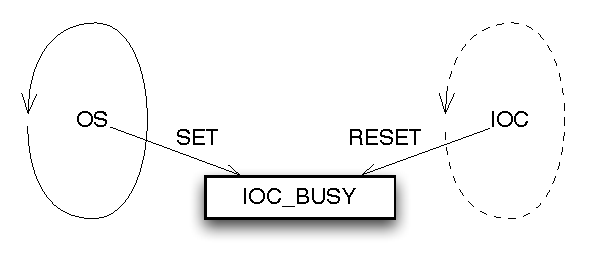
\includegraphics[scale=.75]{diagrammes/IOC-OS}
	\caption{Synchronisation entre IOC et OS}
\end{figure}

\begin{rem*}
	Ce mécanisme est un mécanisme de synchronisation par variable SET / RESET.
	Ce mécanisme est identique à celui utilisé pour le TTY avec le registre \lstinline!TTY_STATUS!.
\end{rem*}

Le contrôleur de disque IOC présenté ici ne peut exécuter qu'un seul transfert entre la mémoire et le disque à la fois. 

\begin{wrapfigure}{r}{0.40\textwidth}
	\vspace{-15pt}
	\begin{center}
		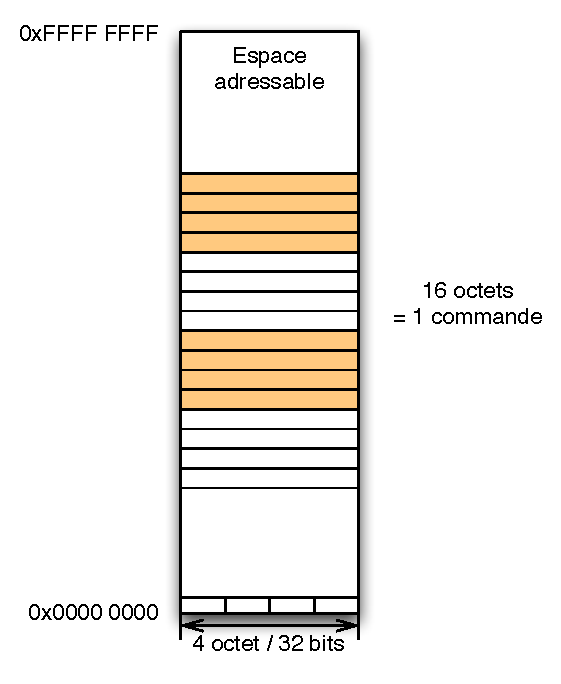
\includegraphics[width=0.30\textwidth]{diagrammes/file_attente}
		\vspace{-15pt}
	\end{center}
	
\end{wrapfigure}

Pour éviter de rendre bloquant (ie. l'appel système entre dans une boucle d'attente active \lstinline!ioc_completed! où l'attente peut être longue) les appels systèmes \lstinline!ioc_read! et \lstinline!ioc_write!, l'OS peut stocker les paramètres de la commande dans une file d'attente en mémoire.

Pour ce faire, il réserve des paquets de 16 octets dans l'espace adressable où chaque paquet représente une commande en attente.

Objectif. Eviter au processeur de gâcher des cycles en faisant de l'attente active.

Dans les contrôleurs IOC les plus récents, la file d'attente des commandes de transfert est une structure de données (file de type FIFO) partagée entre l'OS et l'IOC (variable de synchronisation nécessaire).

\clearpage
\section{Architecture matérielle finale} % (fold)

\begin{figure}[!h]
	\center
	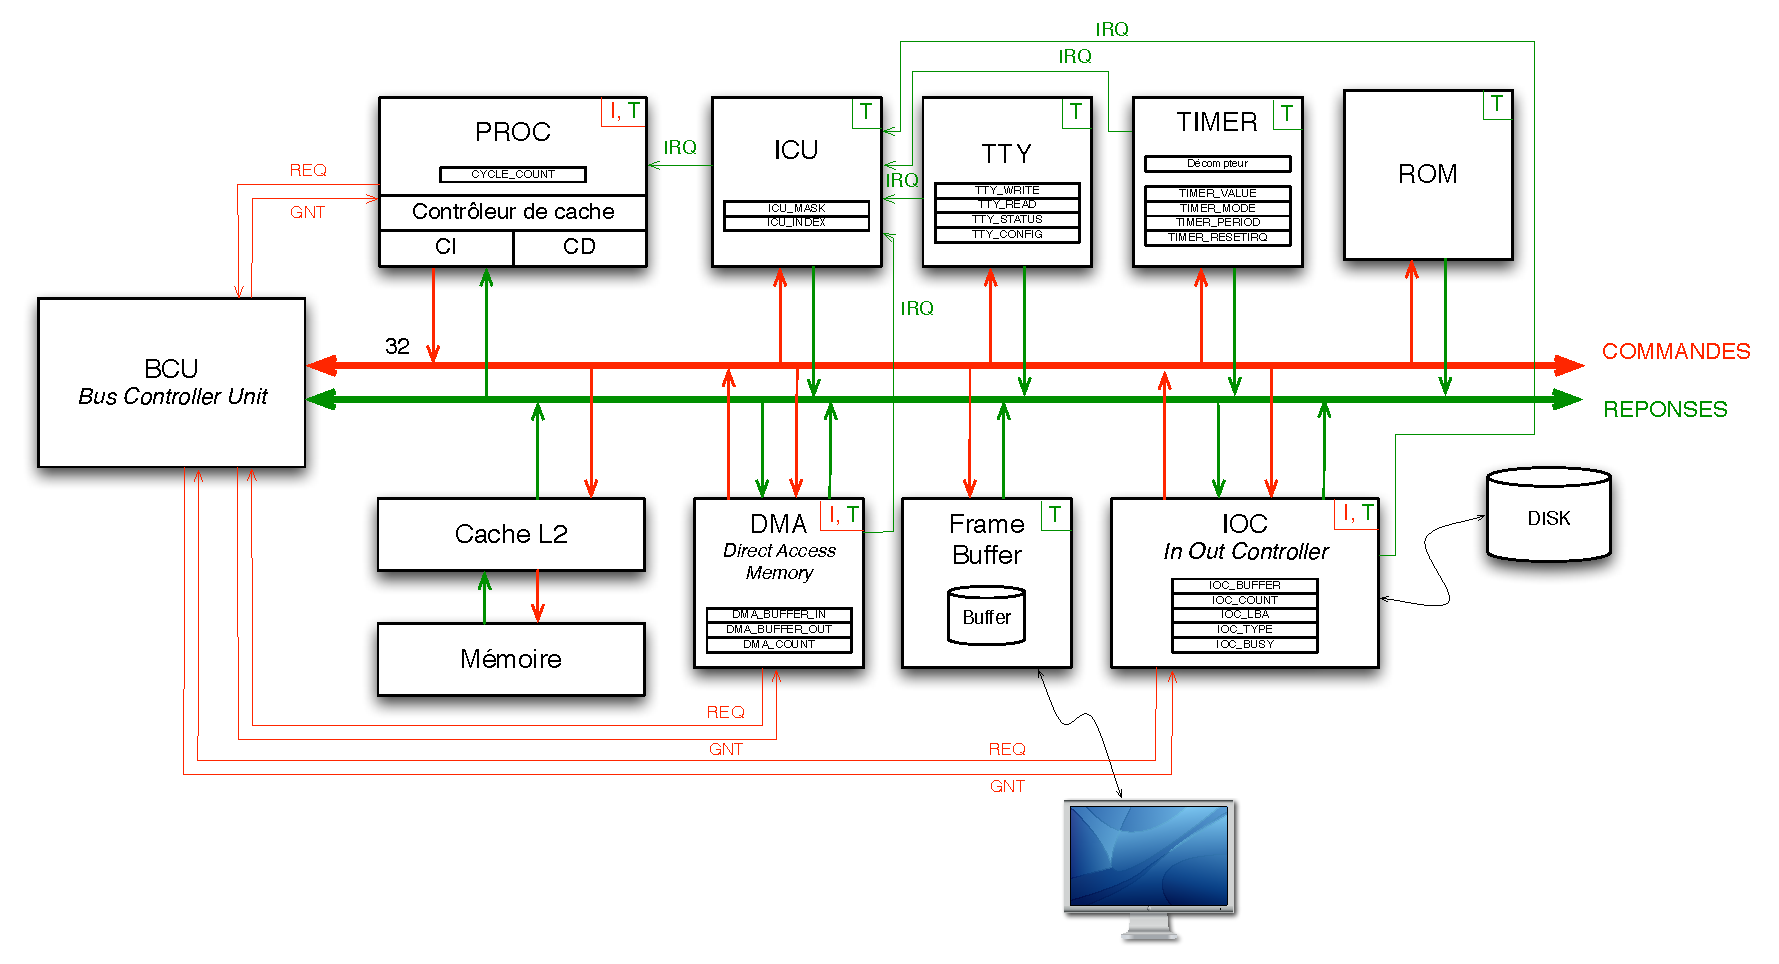
\includegraphics[scale=.60]{diagrammes/architecture-finale}
	\caption{Architecture matérielle ALMO5}
\end{figure}

\subsection{DMA (\emph{Direct Memory Access})} % (fold)

Le composant « DMA » est utilisé pour déplacer des données, d’un tampon mémoire source vers un tampon mémoire destination. 

C’est un maître sur le bus puisqu’il est capable de lire et d’écrire à n’importe quelle adresse dans l’espace adressable du système. 

C’est également une cible, puisqu’il contient un (petit) nombre de registres adressables dans lesquels le système d’exploitation peut écrire, pour définir les caractéristiques du transfert à effectuer (adresse du tampon source, adresse du tampon destination, nombre d’octets à transférer). Une fois configuré, ce composant travaille en parallèle avec le processeur, et signale la fin du transfert en activant une ligne d’interruption spécifique.

Le composant DMA contient alors 3 registres adressables :\begin{itemize}
	\item Adresse tampon source \lstinline!DMA_BUFFER_IN! ;
	\item Adresse tampon destination \lstinline!DMA_BUFFER_OUT! ;
	\item Nombre d'octets à transférer \lstinline!DMA_COUNT!.
\end{itemize}

\subsection{Block I/O ou IOC (\emph{In Out Controller})} % (fold)

Le composant « Block I/O » est un contrôleur de disque. Il est utilisé pour transférer des données entre un tampon mémoire et un fichier situé sur un composant de stockage externe tel qu’un disque magnétique. Tous les transferts se font par blocs de 512 octets (appelés « secteurs » dans le cas des disques). 

Le contrôleur de disque est aussi un maître sur le bus puisqu’il capable de lire et d’écrire en mémoire à n’importe quelle adresse dans l’espace adressable. 

C’est également une cible, puisqu’il contient un (petit) nombre de registres adressables dans lesquels le système d’exploitation peut écrire, pour définir le transfert à effectuer (adresse du tampon en mémoire, désignation du premier bloc dans le fichier, nombre de blocs à transférer). Une fois configuré, ce composant travaille en parallèle avec le processeur, et signale la fin du transfert en activant sa propre ligne d’interruption.

\subsection{Frame Buffer} % (fold)

Le composant « Frame Buffer » est un contrôleur vidéo permettant d’afficher des images sur un écran graphique. Ce composant contient une mémoire vidéo permettant de stocker une image de dimension prédéfinie. On s’intéressera à des images en « niveaux de gris ». Chaque pixel est codé sur un octet. Il y a donc 256 niveaux de gris, et la valeur 0 correspond à un pixel noir. Pour avoir des temps d’exécution raisonnables, on se limite à des images de 128 lignes de 128 pixels. 

Dans un PC, la capacité de la mémoire vidéo atteint couramment 4 Moctets (1024 lignes de 1024 bits, chaque pixel étant codé sur 4 octets pour l’affichage couleur. Cette mémoire vidéo est parcourue à une fréquence fixe (typiquement 25 fois par seconde) de façon à générer le signal vidéo qui est envoyé vers le terminal graphique. Cette mémoire vidéo (ou « frame buffer ») est généralement implantée dans la partie de l’espace adressable réservée au système d’exploitation. 

Le « Frame Buffer » est un composant cible sur le bus. Il ne possède pas de registres adressables.

\begin{lstlisting}
/* Fonctions bloquantes */
int fb_sync_write(size_t offset, void* buffer, size_t length);
int fb_sync_read(size_t offset, void* buffer, size_t length);
\end{lstlisting}

Ces deux fonctions effectuent le transfert de façon purement logicielle : chaque octet du tampon source est chargé par le processeur dans un registre interne, puis écrit par le processeur dans le tampon destination. 

Ces fonctions sont bloquantes et ne rendent la main que lorsque le transfert est terminé $\Rightarrow$ transfert est synchrone. Cette technique est simple, mais elle est lente.

\begin{lstlisting}
/* Fonctions non bloqantes */
int fb_write(size_t offset, void* buffer, size_t length);
int fb_read(size_t offset, void* buffer, size_t length);
int fb_completed();
\end{lstlisting}

Les deux fonctions \lstinline!fb_write()! et \lstinline!fb_read()! utilisent le composant matériel DMA pour accélérer le transfert. Le mécanisme est très similaire à celui utilisé par le contrôleur I/O. Ces deux fonctions sont non bloquantes. 

Elles configurent le contrôleur DMA pour que celui-ci effectue le transfert et rendent immédiatement la main au programme utilisateur. Plus tard, le contrôleur DMA active une interruption pour signaler la fin du transfert. 

Comme dans le cas du contrôleur I/O, la fonction \lstinline!fb_completed()! est une fonction bloquante qui ne rend la main que lorsque le transfert est terminé.

On utilise des appels système car il faut invalider les lignes de cache avec la fonction \lstinline!_dcache_buf_invalidate! -- problème si l'on veut afficher une nouvelle image. De plus, il faut vérifier si le programme est en droit de faire l'affichage (ie. adresse < 0x8000 0000).

\chapter{Fonctionnement multitâche} % (fold)

\section{Introduction} % (fold)

\begin{rem*}
	Multitâche $\neq$ multiprocesseur :\begin{itemize}
		\item Multitâche : utilisation de la machine comme si plusieurs programmes s'exécutaient en même temps ;
		\item Multiprocesseur : (au niveau du matériel) une machine peut contenir plusieurs processeurs fonctionnant en parallèle.
	\end{itemize}
\end{rem*}

\begin{def*}[Parallélisme]
	On parle de parallélisme émulé lorsque l'on exécute plusieurs programmes utilisateurs simultanément sur un seul processeur.
\end{def*}

On découpe le temps en tranches de durée fixe (quantum). Arbitrairement : 1 tanche = 10 ms = 10 millions de cycles (1 cycle = $10^{-9}$ s).

\begin{figure}[!h]
	\center
	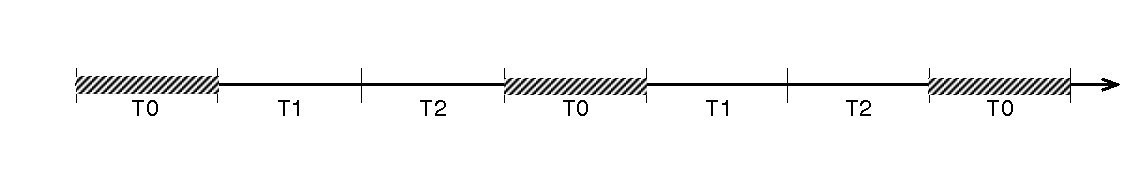
\includegraphics[scale=.75]{diagrammes/tranches}
	\caption{Tranches de temps}
\end{figure}

Dans l'exemple ci-dessus, chaque tâche aura exécuté 33 tranches.
Chaque programme va s'exécuter 3 fois moins vite que s'il avait été seul.

C'est du pseudo-parallélisme par multiplexage temporel.

Les évènements périodiques de changement de contexte (le processeur travaille pour la tâche T0 et passe à la tâche T1) sont générés par un TIMER TICK. Le terme TICK désigne au choix :\begin{itemize}
	\item L'interruption qui déclenche  un changement de contexte ;
	\item La périodicité de l'évènement déclencheur d'un changement de contexte.
\end{itemize}

\begin{def*}[Contexte]
	Ensemble des informations qui doivent être sauvegardées pour permettre à une tâche sortante de recommencer à s'exécuter lorsque ce sera son tour de rentrer (ie. devenir une tâche entrante).
	
	Sauvegarde des registres :\begin{itemize}
		\item Tous les registres généraux R($i$) sauf R(0), R(26) et R(27) (registres réservés au système) ;
		\item EPC (PC sauvegardé dans EPC), \lstinline!STATUS REGISTER! (SR), \lstinline!CAUSE REGISTER! (CR), HI, LO.
	\end{itemize}
\end{def*}

\begin{rem*}
	Ce système de sauvegarde des registres est similaire à celui de la sauvegarde du contexte d'exécution d'une fonction.
	
	Chaque tâche ayant sa propre pile, il suffit de sauvegarder le pointeur de pile R(29).
\end{rem*}
\begin{wrapfigure}{r}{0.37\textwidth}
	\center
	\vspace{-40pt}
	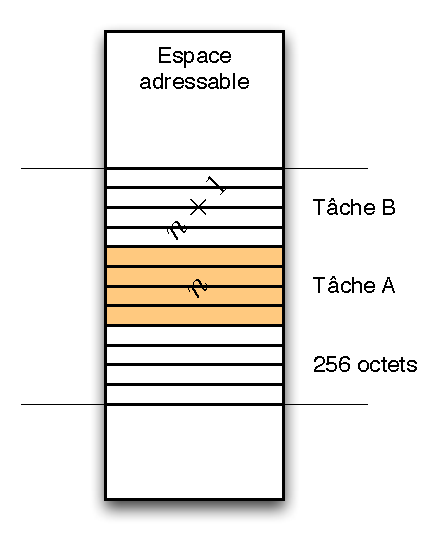
\includegraphics[scale=.5]{diagrammes/taches}
	\vspace{-35pt}
\end{wrapfigure}
L'OS a besoin de stocker en mémoire \textbf{les} contextes d'exécution des $N$ tâches en cours d'exécution (1 contexte = 32-3+5 = 34 registres de 32 bits). L'OS possède donc un ``tableau de contextes'' où  chaque ``case'' de ce tableau a une capacité de 256 octets.

L'OS a besoin d'une case mémoire permettant de stocker le numéro du programme utilisateur en cours d'exécution.


\section{Mécanisme de changement de contexte} % (fold)

\begin{figure}[!h]
	\center
	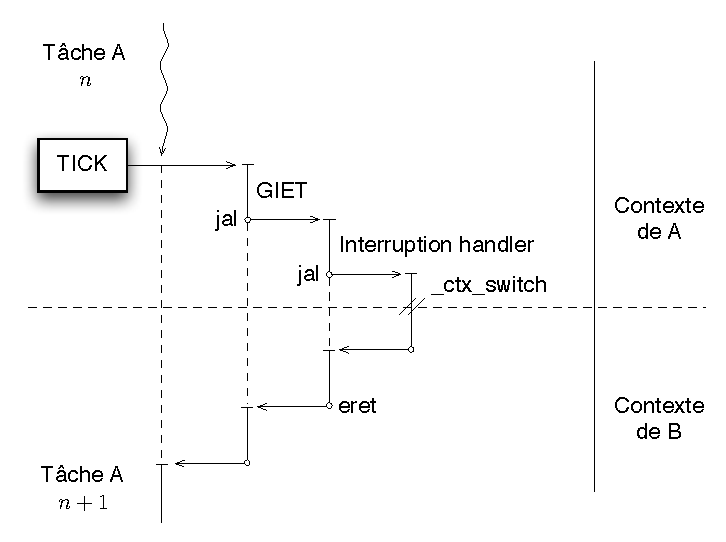
\includegraphics[scale=.75]{diagrammes/ctx_switch}
	\caption{Changement de contexte}
\end{figure}

Au moment du TICK (ie. le TIMER génère une IRQ) :\begin{itemize}
	\item Point d'entrée du GIET (0x8000 0180) ;
	\item Le registre CR contient le code d'une interruption : branchement à la fonction \lstinline!_int_handler! ;
	\item Le registre \lstinline!ICU_INDEX! contient le numéro de l'entrée d'interruption \lstinline!IRQ_IN!  associée au TIMER ;
	\item Exécution de l'ISR associée au TIMER \lstinline!_isr_switch! ;
	\item Branchement à la fonction \lstinline!_ctx_switch! ;
\end{itemize}

\begin{rem*}
	Les tâches sont élues suivant l'algorithme \emph{Round Robin} qui assigne des portions de temps égales pour chaque tâche et exécute toutes les tâches sans priorité, dans un ordre cyclique. 
\end{rem*}

\begin{rem*}
	Dans le GIET, on ne peut pas créer \emph{dynamiquement} des tâches ; la création de tâches est réalisée \emph{statiquement} dans la phase de BOOT.
	
	Phase de BOOT :\begin{itemize}
		\item Initialisation des registres (pile, SR) ;
		\item Initialisation des périphériques ;
		\item Initialisation de la tâche principale ;
		\item Initialisation des tableaux de contexte des autres tâches qui démarrent au TICK.
	\end{itemize}
\end{rem*}

\begin{def*}[Virtualisation]
	Donner l'impression à l'utilisateur qu'il y a plus de ressources que réellement.
	
	Le fonctionnement multitâche consiste à utiliser un seul processeur physique (matériel) comme $n$ processeurs virtuels.
\end{def*}

Pour permettre à plusieurs applications de s'exécuter en pseudo-parallélisme, il faut :\begin{itemize}
	\item Partager le processeur (ie. virtualiser le processeur) ;
	\item Partager la mémoire.
\end{itemize}

La \textbf{mémoire virtuelle} consiste à donner à chaque application l'impression qu'elle dispose de la totalité de l'\textbf{espace adressable}. Ce mécanisme permet de compiler chaque application comme si elle s'exécutait seule sur la machine.

\begin{def*}[Adresse logique vs. adresse physique]
	Les adresses logiques (virtuelles) sont les adresses calculées par le compilateur (lors de l'édition de liens) que l'on retrouve dans le code binaire (fichier exécutable). Ce sont les adresses qui sont émises par le processeur. Une adresse physique permet de référencer, manipuler de la mémoire physique.
	
	Les adresses logiques sont alors traduites en adresses physiques (réelles) au moment de sortir du processeur : entre le processeur et le cache $\Rightarrow$ dans le MMU (\emph{Memory Management Unit}).
\end{def*}

\begin{figure}[!h]
	\center
	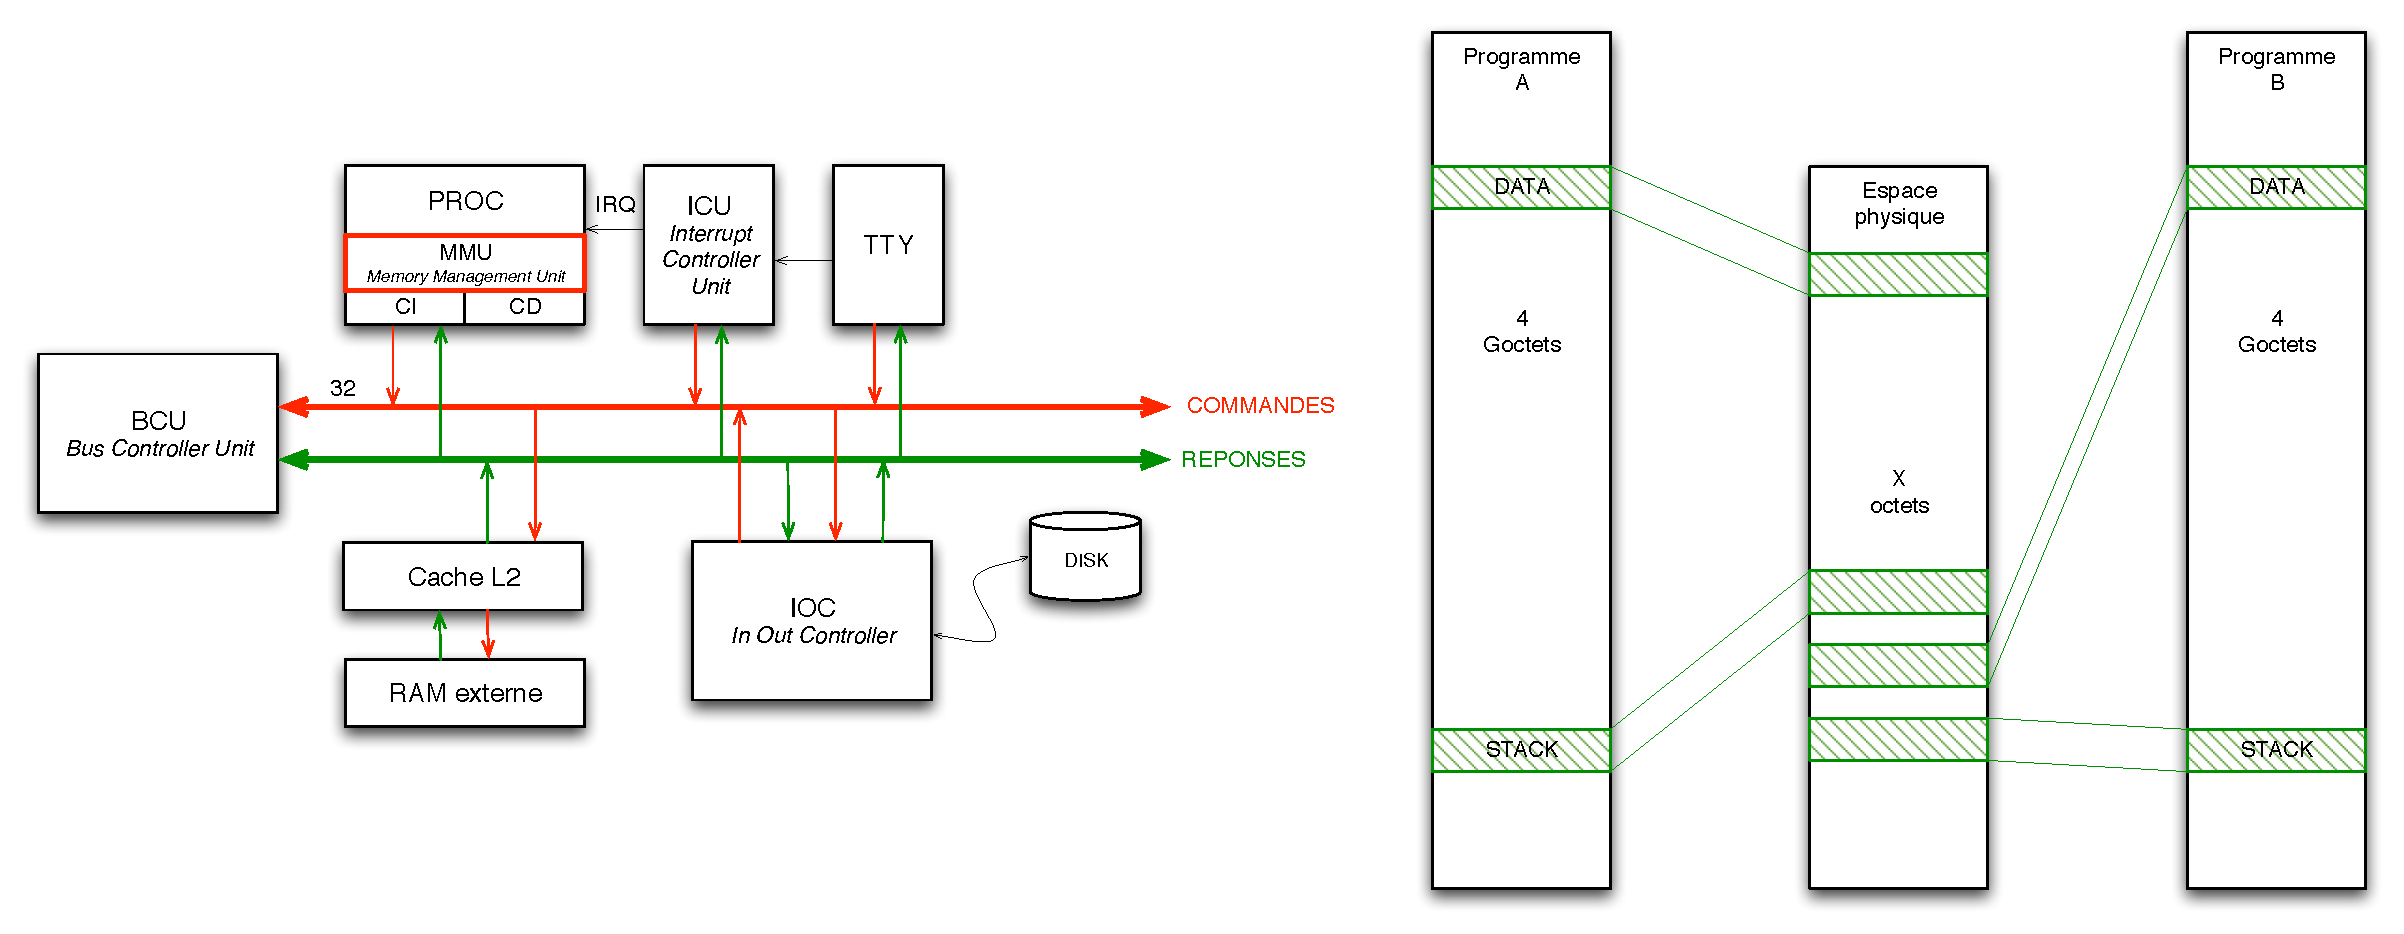
\includegraphics[scale=.40]{diagrammes/MMU}
	\caption{MMU (\emph{Memory Management Unit})}
\end{figure}

Le composant matériel MMU est chargé de faire la traduction ``à la volée'' des \textbf{adresses logiques} vers les \textbf{adresses physiques} (ie. à chaque instruction où le processeur va lire dans le cache, il faut faire une traduction en 1 cycle de l'adresse d'instruction ou de donnée).

Ce composant matériel utilise \textbf{des} tables de traduction : une table de traduction différente pour chaque programme.

Les tables de traduction sont stockées en mémoire ; elles sont chargées lors de la phase de BOOT.

Il n'y a pas de collisions : lorsque l'OS reçoit la demande d'un programme pour accéder aux ressources de la machine, il détermine les segments physiques (STACK, DATA, CODE)  sans collision.

Il faut alors :\begin{itemize}
	\item Un système de \textbf{tables} de traduction ou table de pages (en mémoire) ;
	\item Un composant matériel MMU capable d'utiliser ces tables.
\end{itemize}

La technique moderne de virtualisation de la mémoire est la \textbf{pagination}. 

\begin{def*}[Page]
	Une page est un bloc d'adresses consécutives dans l'espace adressable (logique ou physique) aligné et de taille fixe : 4Ko.
\end{def*}

\begin{rem*}
	Un bloc aligné : l'adresse la plus élevée est un multiple de l'adresse la plus petite.
\end{rem*}

\begin{figure}[!h]
	\center
	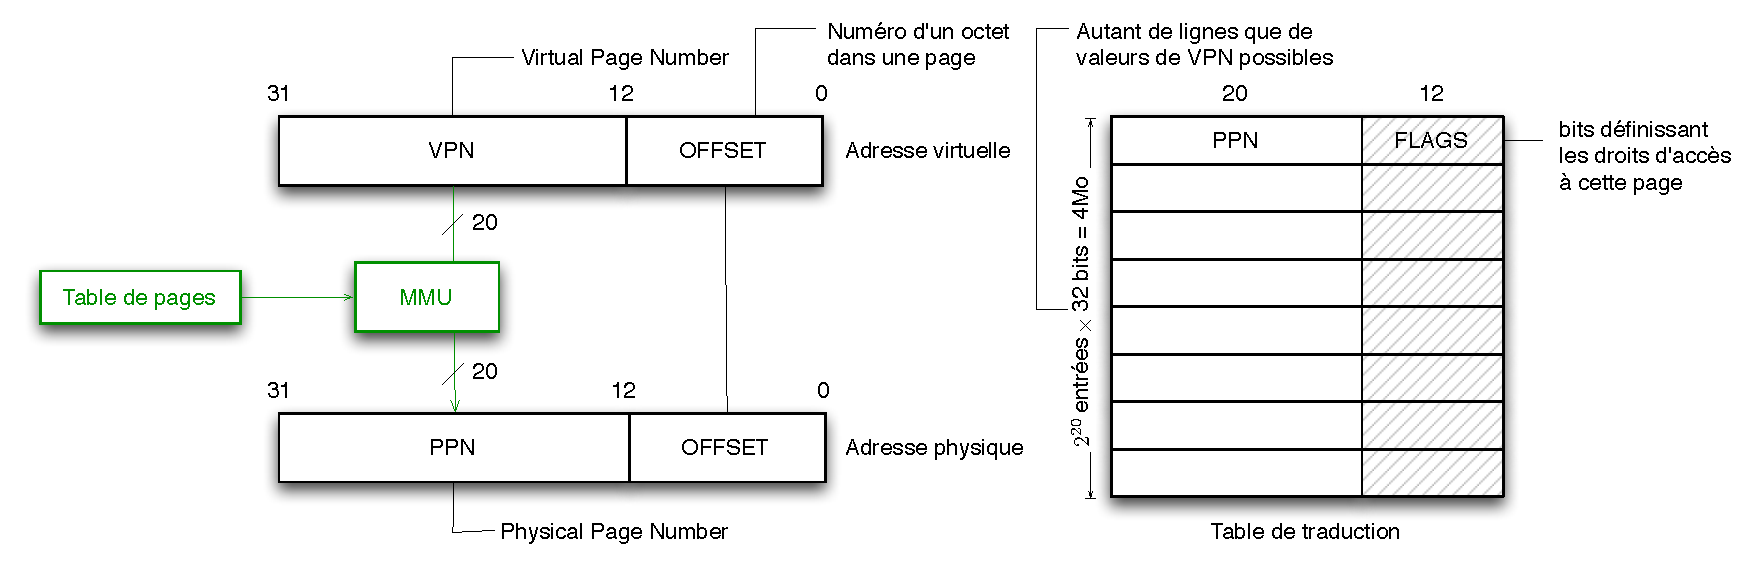
\includegraphics[scale=.60]{diagrammes/VPN_PPN}
	\caption{Lien entre adresse physique et adresse virtuelle}
\end{figure}

Il y a défaut de page lorsqu'un VPN n'est pas associée à un PPN dans la table de pages de la MMU. Il y a alors une erreur de traduction d'adresse virtuelle. Il y a une levée d'exception et l'OS doit alors effectuer un \emph{mapping} pour associer un PPN au VPN recherché en trouvant une page de libre.\\
\textbf{Attention.} Un défaut de page est différent d'un MISS de cache.

La plupart des programmes utilisateurs n'utilisent d'une toute petite partie de leur espace adressable virtuel (ie. 2 Go). De ce fait, la plupart des ``tables de pages'' (ou ``tables de traduction'') sont creuses (ie. contiennent majoritairement des 0).

En général, l'OS utilise des pages à deux niveaux.
\begin{figure}[!h]
	\center
	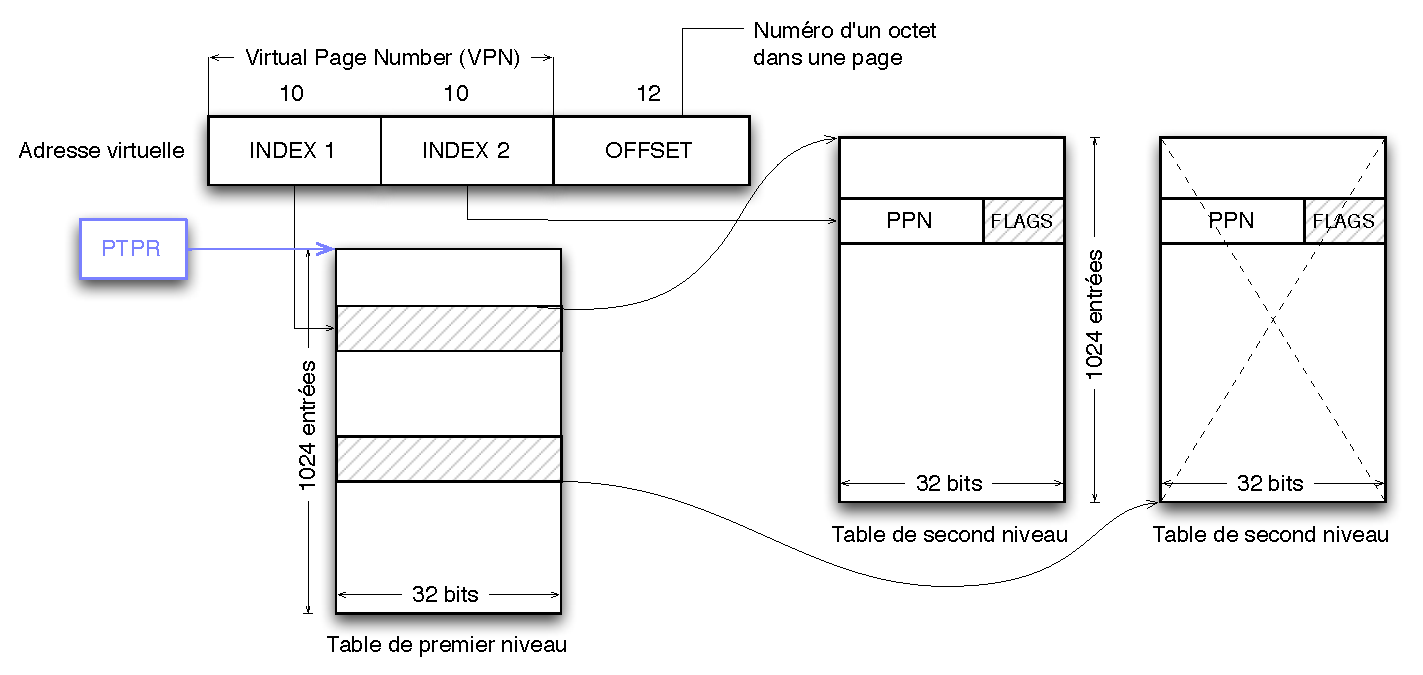
\includegraphics[scale=.60]{diagrammes/pagination_2_niv}
	\caption{Pagination à deux niveaux}
\end{figure}

L'OS ne crée que les tables de pages de 2\ieme niveau qui sont effectivement utilisées.\\
La traduction va alors nécessiter \textbf{deux} lectures mémoire au lieu d'une.

\begin{rem*}
	Le registre PTPR (\emph{Patch Table Pointer Register}) contenu dans le co-processeur contient l'adresse de base de la table de traduction de premier niveau.
\end{rem*}

On gagne de la mémoire et on ralenti le mécanisme de traduction. Une ``vraie'' traduction (effective) coûte au moins deux lectures (environ 30 cycles).

La solution est de placer dans la MMU un petit cache spécialisé : TLB (\emph{Translation Look-aside Buffer}) qui utilise le principe de localité. En effet, puisque les changements de pages sont rares, on en profite pour conserver dans le TLB de la MMU les résultats des dernières traductions.

\begin{def*}[TLB -- \emph{Translation Look-aside Buffer}]
	La TLB permet de conserver localement dans la MMU le résultat de quelques traductions VPN $\rightarrow$ PPN.
	
	La TLB est un tableau associatif (ie. un extrait peut être rangé dans n'importe quelle case $\neq$ cache à correspondance directe : une ligne de cache ne peut être contenue que dans une seule et unique case).
	\begin{figure}[!h]
		\center
		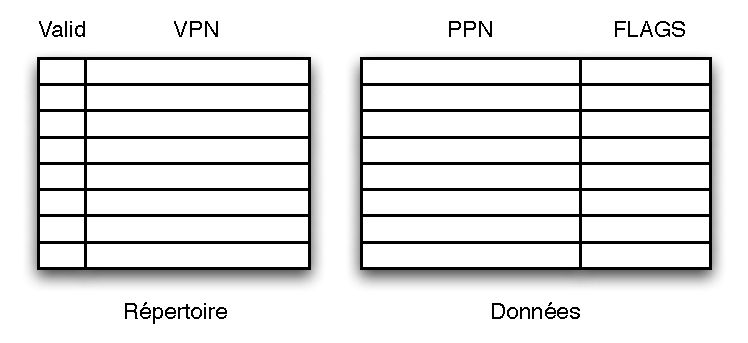
\includegraphics[scale=.60]{diagrammes/TLB}
		\caption{TLB (\emph{Translation Look-aside Buffer})}
	\end{figure}
\end{def*}

Lors d'un MISS TLB, il faut récupérer la correspondance VPN $\leftrightarrow$ PPN en effectuant 2 lectures des tables de traduction.\\
La TLB a un taux de MISS d'environ $10^{-3}$. En cas de MISS sur la TLB, il faut aller consulter les tables de pages en mémoire.

\begin{rem*}
	Lors d'un changement de contexte, il faut :\begin{itemize}
		\item Mettre à jour le registre PTPR ;
		\item Purger la TLB.
	\end{itemize}
	De même qu'il y a deux caches séparés pour les instructions et données (CI et CD), il y a deux TLB pour paralléliser les traductions.
	
	En effet, s'il n'y a qu'un seul cache, pour une lecture de donnée, on perd deux cycles : \begin{itemize}
		\item Lecture de l'instruction ;
		\item Lecture de la donnée.
	\end{itemize}
\end{rem*}

\begin{figure}[h]
	\center
	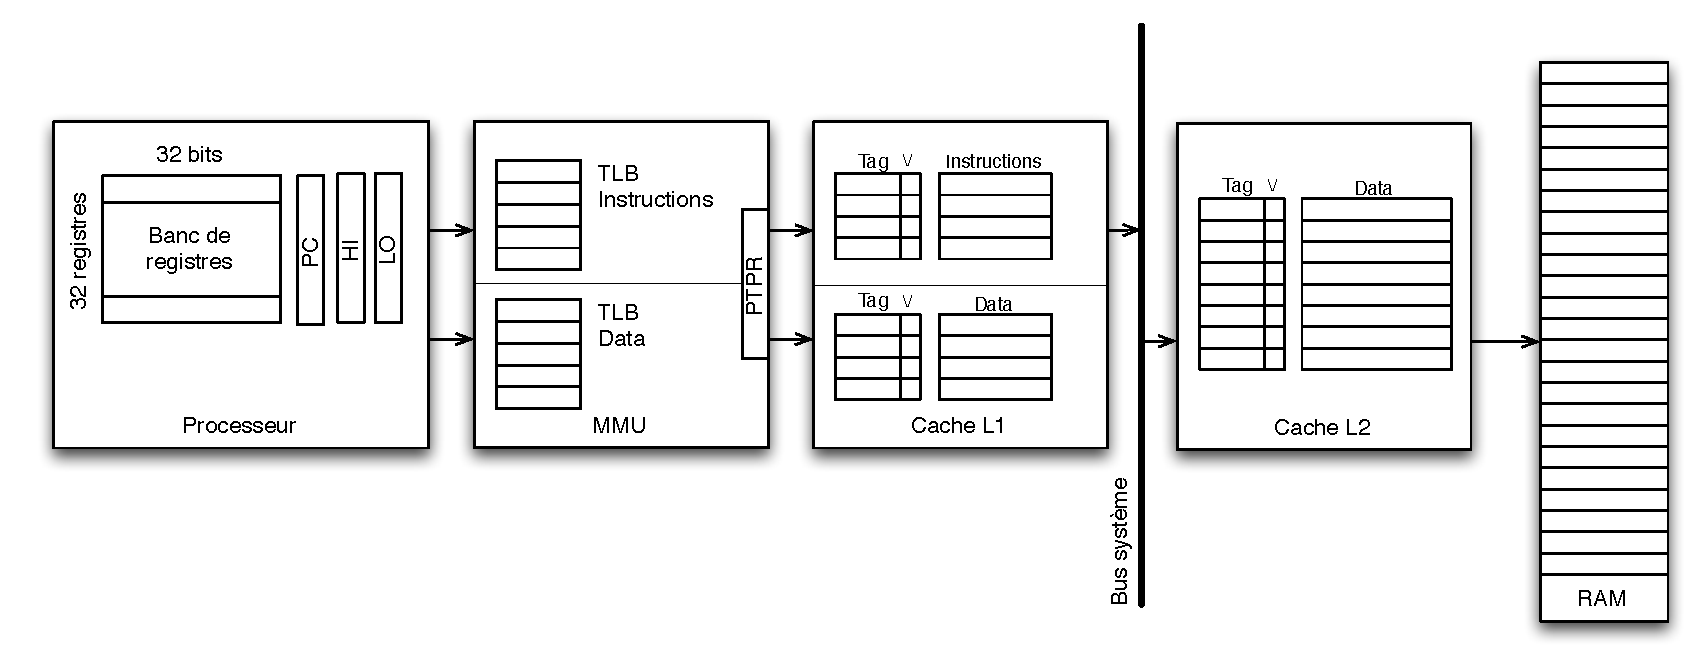
\includegraphics[scale=.59]{diagrammes/hierarchie-mem}
	\caption{Hiérarchie mémoire}
\end{figure}

\chapter{A propos de l'architecture interne des processeurs} % (fold)

\emph{Comment le processeur peut-il exécuter une instruction à chaque cycle ?}

\begin{ex*}
	Soit l'instruction \lstinline!lw $d, $s(imd)  # $d <- M[$s + IMD]!\\
	Cette instruction utilise le processeur pour :\begin{enumerate}
		\item Lire l'instruction en mémoire (IF -- \emph{Instruction Fetch}) ;
		\item Décoder le CODOP (DC -- \emph{DeCode}) ;
		\item Calculer l'adresse \lstinline!$s + IMD! (EX -- \emph{EXecute}) ;
		\item Lecture de la donnée en mémoire (MD -- \emph{Memory Data}) ;
		\item Rangement de la donnée dans \lstinline!$d! (WB -- \emph{Write-back}) ;
		\item PC $\leftarrow$ PC + 4.
	\end{enumerate}
\end{ex*}

La durée réelle d'exécution d'une instruction est de 5 cycles.

\section{Réalisation ``monoprogrammée''} % (fold)
Dans une réalisation ``monoprogrammée'', le processeur est considéré comme un automate, capable d'effectuer une seule instruction à la fois.

\begin{figure}[!h]
	\center
	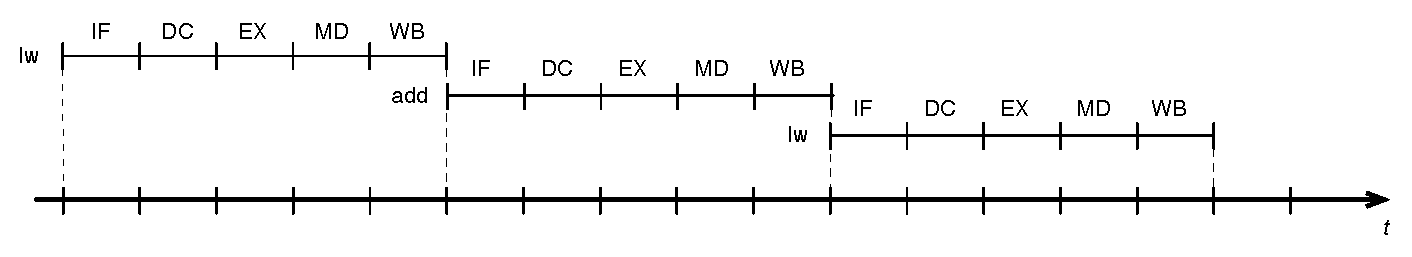
\includegraphics[scale=.60]{diagrammes/monoprogrammee}
\end{figure}

\section{Réalisation ``RISC pipe-line''} % (fold)
Dans une réalisation ``RISC pipe-line'', le processeur n'attend pas d'avoir terminé la dernière étape de l'instruction $i$ pour commencer à exécuter l'instruction $i+1$.

\begin{figure}[!h]
	\center
	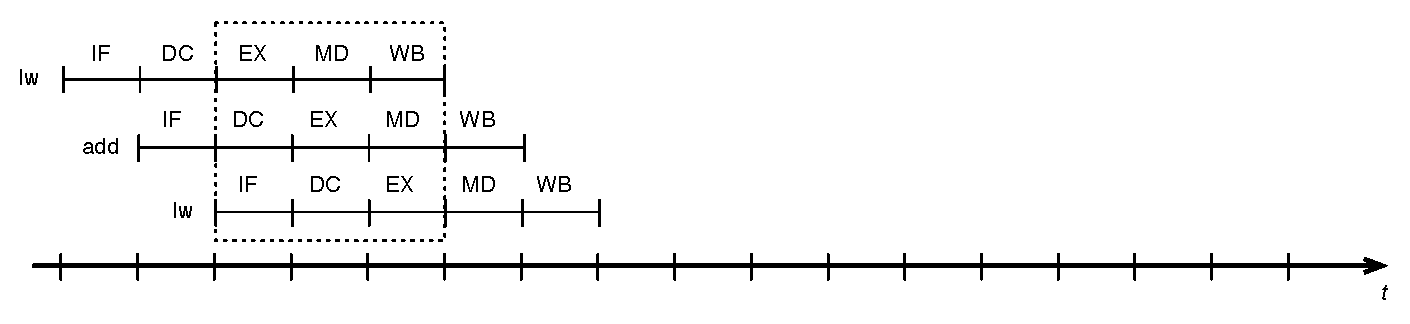
\includegraphics[scale=.60]{diagrammes/RISC-pipe-line}
\end{figure}

\clearpage

\end{document}
